% !TEX program = xelatex
% ============================================================================
% មគ្គុទ្ទេសក៍គរុកោសល្យគ្រូ និងសេណារីយ៉ូបង្រៀនលម្អិត (Teacher's Guideline -- ISO)
% មុខវិជ្ជា៖ គណិតវិទ្យា ថ្នាក់ទី៨ -- មេរៀនទី១២៖ ការប្រៀបធៀបត្រីកោណ
% ចំណុចរង៖ ២.២ លក្ខណៈត្រីកោណសមបាទ និងប្រសព្វមេដ្យាទ័រ (ទំ.១៥៧--១៥៨ & ១៦៤--១៦៥: #2, #8, #11)
% គ្រូបង្រៀន៖ ហុក ប៊ុនថែន | អនុវិទ្យាល័យព្រះក្រសាំង (កំពង់ស្វាយ-កំពង់ធំ)
% ============================================================================
\documentclass[a4paper,12pt]{article}

\usepackage[a4paper, left=1.55cm, right=1.55cm, top=2.30cm, bottom=2.30cm, headheight=20pt, headsep=0.68cm, footskip=0.88cm]{geometry}
\usepackage{amsmath, amssymb}
\usepackage{unicode-math}
\usepackage{fontspec}
\usepackage{array, longtable, multirow, colortbl, booktabs}
\usepackage[table]{xcolor}
\usepackage{enumitem}
\usepackage{pifont}
\usepackage{fancyhdr}
\usepackage{lastpage}
\usepackage{needspace}
\usepackage[hyphens]{url}
\usepackage{tikz}
\usepackage[most]{tcolorbox}
\usetikzlibrary{calc, arrows.meta, angles, quotes, decorations.markings, positioning, babel}
\urlstyle{same}

\makeatletter
\let\@expl@@@mark@update@singlecol@structures@@\relax
\makeatother

% ============================================================================
% ការកំណត់ពុម្ពអក្សរ (Word-Styled Khmer + Times New Roman APA + Cambria Math)
% ============================================================================
% Cross-platform font path resolver (Windows local + Linux/Cloud repo fonts/)
\providecommand{\NGSFindFonts}{%
  \IfFileExists{C:/Windows/Fonts/cambria.ttc}{%
    \def\NGSSysPath{C:/Windows/Fonts/}%
    \def\NGSUserPath{C:/Users/KIT/AppData/Local/Microsoft/Windows/Fonts/}%
  }{%
    \IfFileExists{./fonts/KhmerOSsiemreap.ttf}{\def\NGSSysPath{./fonts/}\def\NGSUserPath{./fonts/}}{%
    \IfFileExists{../fonts/KhmerOSsiemreap.ttf}{\def\NGSSysPath{../fonts/}\def\NGSUserPath{../fonts/}}{%
    \IfFileExists{../../fonts/KhmerOSsiemreap.ttf}{\def\NGSSysPath{../../fonts/}\def\NGSUserPath{../../fonts/}}{%
    \IfFileExists{../../../fonts/KhmerOSsiemreap.ttf}{\def\NGSSysPath{../../../fonts/}\def\NGSUserPath{../../../fonts/}}{%
    \IfFileExists{../../../../fonts/KhmerOSsiemreap.ttf}{\def\NGSSysPath{../../../../fonts/}\def\NGSUserPath{../../../../fonts/}}{%
    \IfFileExists{../../../../../fonts/KhmerOSsiemreap.ttf}{\def\NGSSysPath{../../../../../fonts/}\def\NGSUserPath{../../../../../fonts/}}{%
    \IfFileExists{../../../../../../fonts/KhmerOSsiemreap.ttf}{\def\NGSSysPath{../../../../../../fonts/}\def\NGSUserPath{../../../../../../fonts/}}{%
      \def\NGSSysPath{../../../../../../../fonts/}\def\NGSUserPath{../../../../../../../fonts/}%
    }}}}}}}%
  }%
}
\NGSFindFonts

\setmathfont[
  Path={\NGSSysPath},
  FontIndex=1,
  Scale=1.06
]{cambria.ttc}

\defaultfontfeatures{Ligatures=TeX}

\setmainfont[
  Path={\NGSUserPath},
  Extension=.ttf,
  Script=Khmer,
  BoldFont={KhmerOSsiemreap},
  BoldFeatures={FakeBold=1.8},
  ItalicFont={KhmerOSsiemreap},
  ItalicFeatures={FakeSlant=0.25},
  BoldItalicFont={KhmerOSsiemreap},
  BoldItalicFeatures={FakeBold=1.8, FakeSlant=0.25}
]{KhmerOSsiemreap}

% ហាមដាក់ FakeBold លើ KhmerOSmuollight និងកុំរុំ \muol ក្នុង \textbf{...}
\newfontfamily\muol[
  Path={\NGSUserPath},
  Extension=.ttf,
  Script=Khmer
]{KhmerOSmuollight}

\newfontfamily\TimesEn[
  Path={\NGSSysPath},
  Extension=.ttf,
  Scale=1.02,
  BoldFont={timesbd},
  ItalicFont={timesi},
  BoldItalicFont={timesbi}
]{times}

\newfontfamily\Tacteing[
  Path={\NGSUserPath}
]{TACTENG.TTF}

\newfontfamily\CourierBullet[
  Path={\NGSSysPath},
  Extension=.ttf
]{cour}

% ក្បួនកាត់ពាក្យខ្មែរ (Khmer word wrapping)
\XeTeXlinebreaklocale "km"
\XeTeXlinebreakskip = 0pt plus 1pt minus 0.1pt

% Mobile-First comfortable line spacing (11.5pt / 18.2pt effective)
\linespread{1.22}

% ============================================================================
% ពណ៌ ស-ខ្មៅ (Strict Monochrome Grayscale Palette) & Fancyhdr
% ============================================================================
\definecolor{headgray}{HTML}{F2F2F2}
\definecolor{panelgray}{gray}{0.94}
\definecolor{stepgray}{HTML}{D9D9D9}
\definecolor{midgray}{gray}{0.82}
\definecolor{bordergray}{gray}{0.45}

\pagestyle{fancy}
\fancyhf{}
\renewcommand{\headrulewidth}{0.4pt}
\renewcommand{\footrulewidth}{0.4pt}
\fancyhead[L]{\rule[-3pt]{0pt}{14pt}\fontsize{9.2pt}{13pt}\selectfont មគ្គុទ្ទេសក៍គរុកោសល្យគ្រូ \en{(Grade 8 ISO)}}
\fancyhead[R]{\rule[-3pt]{0pt}{14pt}\fontsize{9.2pt}{13pt}\selectfont មេរៀនទី១២ \en{(}២.២\en{)}៖ ត្រីកោណសមបាទ និងប្រសព្វមេដ្យាទ័រ}
\fancyfoot[L]{\rule{0pt}{13pt}\fontsize{9.8pt}{13.5pt}\selectfont កញ្ចប់ឯកសារ \en{NGS 5Es} \en{(}៥០ នាទី\en{)} \en{|} ហុក ប៊ុនថែន}
\fancyfoot[R]{\rule{0pt}{13pt}\fontsize{9.8pt}{13.5pt}\selectfont ទំព័រ \en{\thepage\ / \pageref{LastPage}}}

\fancypagestyle{firstpage}{%
  \fancyhf{}%
  \renewcommand{\headrulewidth}{0pt}%
  \renewcommand{\footrulewidth}{0.4pt}%
  \fancyfoot[L]{\rule{0pt}{13pt}\fontsize{9.8pt}{13.5pt}\selectfont កញ្ចប់ឯកសារ \en{NGS 5Es} \en{(}៥០ នាទី\en{)} \en{|} អនុវិទ្យាល័យព្រះក្រសាំង}%
  \fancyfoot[R]{\rule{0pt}{13pt}\fontsize{9.8pt}{13.5pt}\selectfont ទំព័រ \en{\thepage\ / \pageref{LastPage}}}%
}

\setlength{\parindent}{0pt}
\setlength{\parskip}{3.0pt}
\setlength{\tabcolsep}{4pt}
\setlength{\emergencystretch}{2em}
\setlist{itemsep=2.5pt, parsep=0pt}

% ============================================================================
% ម៉ាក្រូជំនួយ និងឋានានុក្រម \muol គ្មានតួអក្សរ ASCII បន្លំ
% ============================================================================
\newcommand{\en}[1]{{\TimesEn #1}}
\newcommand{\enbf}[1]{{\TimesEn\textbf{#1}}}
\newcommand{\enit}[1]{{\TimesEn\textit{#1}}}
\newcommand{\unit}[1]{\,\text{\en{#1}}}
\newcommand{\cnum}[1]{{\TimesEn\fontsize{10.5pt}{12pt}\selectfont\ding{\numexpr181+#1\relax}}}
\newcommand{\ditem}{\tikz[baseline=-0.5ex]\fill (0,0.40ex) -- (0.40ex,0) -- (0,-0.40ex) -- (-0.40ex,0) -- cycle;\hspace{0.25em}}
\newcommand{\wcirc}{{\CourierBullet\fontsize{9.8pt}{11pt}\selectfont o}}
\newcommand{\chkbox}{\tikz[baseline=-0.15ex]\draw[black, line width=0.85pt] (0,0) rectangle (0.25cm,0.25cm);}
\newcommand{\tri}[1]{\ensuremath{\triangle #1}}
\newcommand{\ang}[1]{\ensuremath{\angle #1}}
\newcommand{\cg}{\ensuremath{\cong}}
\newcommand{\ncg}{\ensuremath{\not\cong}}
\newcommand{\khmflourish}{{\Tacteing\fontsize{38pt}{15pt}\selectfont\raisebox{-5pt}{3}}}
\newcommand{\tickone}{\tikz[baseline=-0.2ex]\draw[black, line width=1.1pt] (0,0.02cm) -- (0.06cm,0.23cm);}
\newcommand{\ticktwo}{\tikz[baseline=-0.2ex]{\draw[black, line width=1.1pt] (0,0) -- (0,0.24cm);\draw[black, line width=1.1pt] (0.08cm,0) -- (0.08cm,0.24cm);}}
\newcommand{\tickthree}{\tikz[baseline=-0.2ex]{\draw[black, line width=1.1pt] (0,0) -- (0,0.24cm);\draw[black, line width=1.1pt] (0.07cm,0) -- (0.07cm,0.24cm);\draw[black, line width=1.1pt] (0.14cm,0) -- (0.14cm,0.24cm);}}

\newcommand{\parttitle}[1]{{\muol\fontsize{13pt}{17pt}\selectfont #1}}
\newcommand{\sectitle}[1]{{\muol\fontsize{12pt}{15.5pt}\selectfont #1}}
\newcommand{\subsectitle}[1]{{\muol\fontsize{11pt}{14.5pt}\selectfont #1}}
\newcommand{\tblhead}[1]{{\muol\fontsize{10.5pt}{16.2pt}\selectfont #1\par}}

\newcolumntype{L}[1]{>{\raggedright\arraybackslash}p{#1}}
\newcolumntype{C}[1]{>{\centering\arraybackslash}p{#1}}
\newcolumntype{R}[1]{>{\raggedleft\arraybackslash}p{#1}}

\newcommand{\secbanner}[2]{%
  \Needspace{2.2cm}%
  \vspace{2pt}%
  \begin{tcolorbox}[
    enhanced, sharp corners, colback=stepgray, colframe=black,
    boxrule=1.1pt, borderline south={0.6pt}{1.8pt}{black},
    top=4.5pt, bottom=4.5pt, left=9pt, right=9pt,
    before skip=5pt, after skip=4pt
  ]
    \sectitle{#1}\\[2pt]
    {\fontsize{10pt}{12.5pt}\selectfont\enit{#2}}%
  \end{tcolorbox}%
}

\newcommand{\refbanner}[1]{%
  \Needspace{2.2cm}%
  \vspace{2pt}%
  \begin{tcolorbox}[
    enhanced, sharp corners, colback=panelgray, colframe=black,
    boxrule=0.85pt, top=6pt, bottom=6pt, left=9pt, right=9pt,
    before skip=6pt, after skip=5pt
  ]
    {\muol\fontsize{12pt}{19pt}\selectfont #1}%
  \end{tcolorbox}%
}

\newcommand{\subsec}[1]{%
  \Needspace{1.6cm}%
  \vspace{3pt}%
  \subsectitle{#1}\par%
  \vspace{-2pt}%
  {\color{black}\hrule height 0.55pt}%
  \vspace{3pt}%
}

\newtcolorbox{phasebox}[3]{%
  enhanced, breakable, sharp corners,
  colback=white, colframe=black,
  boxrule=1.0pt, top=4pt, bottom=4pt, left=9pt, right=9pt,
  toptitle=3pt, bottomtitle=3pt,
  before skip=4.5pt, after skip=0pt,
  colbacktitle=headgray, coltitle=black,
  fonttitle=\fontsize{11pt}{14.5pt}\selectfont,
  fontupper=\fontsize{11.5pt}{14.92pt}\selectfont,
  title={%
    \linespread{1.0}\selectfont\renewcommand{\arraystretch}{1.0}%
    \begin{tabular*}{\linewidth}{@{}>{\raggedright\arraybackslash}p{13.45cm}@{\extracolsep{\fill}}r@{}}
      {\muol\fontsize{11pt}{14.5pt}\selectfont #1} & {\fontsize{10.5pt}{13.5pt}\selectfont\en{#2 |} #3}%
    \end{tabular*}%
  }
}

\newtcolorbox{scriptbox}{%
  enhanced, breakable, sharp corners, colback=panelgray, colframe=black,
  boxrule=0.8pt, borderline west={2.4pt}{0pt}{black},
  top=4.5pt, bottom=4.5pt, left=9pt, right=8pt,
  before skip=-0.8pt, after skip=4.5pt,
  fontupper=\fontsize{11.5pt}{14.92pt}\selectfont
}

\tikzset{
  tk1/.style={postaction={decorate}, decoration={markings, mark=at position 0.50 with {\draw[black, line width=0.95pt] (0,-0.11) -- (0,0.11);}}},
  tk2/.style={postaction={decorate}, decoration={markings,
    mark=at position 0.44 with {\draw[black, line width=0.95pt] (0,-0.11) -- (0,0.11);},
    mark=at position 0.56 with {\draw[black, line width=0.95pt] (0,-0.11) -- (0,0.11);}}},
  tk3/.style={postaction={decorate}, decoration={markings,
    mark=at position 0.41 with {\draw[black, line width=0.95pt] (0,-0.11) -- (0,0.11);},
    mark=at position 0.50 with {\draw[black, line width=0.95pt] (0,-0.11) -- (0,0.11);},
    mark=at position 0.59 with {\draw[black, line width=0.95pt] (0,-0.11) -- (0,0.11);}}},
  hypArrow/.style={black, densely dashed, line width=0.85pt, -{Stealth[length=4pt]}},
  ang1/.style={draw=black, line width=0.8pt}
}

\newcommand{\rightanglemark}[4][0.22]{%
  % #2 = vertex, #3 = point on ray 1, #4 = point on ray 2
  \coordinate (raA) at ($#2!#1cm!#3$);
  \coordinate (raB) at ($#2!#1cm!#4$);
  \coordinate (raC) at ($(raA)+(raB)-#2$);
  \draw[line width=0.8pt, black] (raA) -- (raC) -- (raB);
}

\begin{document}
\thispagestyle{firstpage}
\fontsize{11.5pt}{14.92pt}\selectfont
\vspace*{-0.75cm}

% ============================================================================
% ក្បាលលិខិតផ្លូវការថ្នាក់ជាតិ & សាលារៀន (Kampong Thom / Kampong Svay / Preah Krasang)
% ============================================================================
{\linespread{1.08}\selectfont
\begin{center}
  {\muol\fontsize{12pt}{15.5pt}\selectfont ព្រះរាជាណាចក្រកម្ពុជា}\\[2pt]
  {\muol\fontsize{12pt}{15.5pt}\selectfont ជាតិ សាសនា ព្រះមហាក្សត្រ}\\[1pt]
  \khmflourish
\end{center}
\vspace{-4pt}
{\muol\fontsize{10.8pt}{15.5pt}\selectfont
  មន្ទីរអប់រំ យុវជន និងកីឡា ខេត្តកំពង់ធំ\\
  ការិយាល័យអប់រំ យុវជន និងកីឡា ស្រុកកំពង់ស្វាយ\\
  អនុវិទ្យាល័យព្រះក្រសាំង\par}
\vspace{4pt}
\begin{center}
  \parttitle{មគ្គុទ្ទេសក៍គរុកោសល្យគ្រូ និងសេណារីយ៉ូបង្រៀនលម្អិត \enbf{(Teacher's Guideline)}}\\[3pt]
  {\fontsize{11.2pt}{15pt}\selectfont\textbf{មេរៀនទី១២៖ ការប្រៀបធៀបត្រីកោណ \en{---} ២. មេដ្យាទ័រនៃអង្កត់និងត្រីកោណសមបាទ \en{---} ២.២ លក្ខណៈត្រីកោណសមបាទ និងប្រសព្វមេដ្យាទ័រ}}
\end{center}
}

\vspace{2pt}
\begin{tcolorbox}[
  enhanced, sharp corners, colback=headgray, colframe=black,
  boxrule=0.85pt, top=5pt, bottom=5pt, left=7pt, right=7pt,
  before skip=2pt, after skip=6pt
]
  \linespread{1.10}\fontsize{10.5pt}{14pt}\selectfont
  \renewcommand{\arraystretch}{1.18}
  \begin{tabular}{@{}L{3.10cm}@{}C{0.25cm}@{}L{5.55cm}@{\hspace{0.25cm}}L{2.70cm}@{}C{0.25cm}@{}L{5.00cm}@{}}
    \textbf{\en{-} មុខវិជ្ជា \en{/} ថ្នាក់} & \en{:} & គណិតវិទ្យា \en{(}ថ្នាក់ទី៨\en{)} & \textbf{\en{-} កាលបរិច្ឆេទ} & \en{:} & ថ្ងៃពុធ ទី២ ខែធ្នូ ឆ្នាំ២០២៦ \\
    \textbf{\en{-} ជំពូក \en{/} មេរៀន} & \en{:} & ធរណីមាត្រ \en{/} មេរៀនទី១២ & \textbf{\en{-} រយៈពេល} & \en{:} & ៥០ នាទី \en{(}១ ម៉ោងសិក្សា\en{)} \\
    \textbf{\en{-} ចំណុចរង} & \en{:} & ២.២ ត្រីកោណសមបាទ \& ប្រសព្វ & \textbf{\en{-} សៀវភៅគោល} & \en{:} & ទំ. ១៥៧--១៥៨, ១៦៤--១៦៥ \en{(\#2, \#8, \#11)} \\
    \textbf{\en{-} បង្រៀនដោយ} & \en{:} & ហុក ប៊ុនថែន & \textbf{\en{-} ឯកសារកញ្ចប់} & \en{:} & \en{4 Docs + Open-Access Evidence}
  \end{tabular}
\end{tcolorbox}

% ============================================================================
% ផ្នែកទី ១៖ បរិបទមេរៀន និងទិដ្ឋភាពទូទៅគរុកោសល្យ
% ============================================================================
\secbanner{ផ្នែកទី ១៖ បរិបទមេរៀន និងទិដ្ឋភាពទូទៅគរុកោសល្យ}{Section 1: Administrative Context, Grade 8 Kampong Svay Setting \& 50-Min Isosceles/Circumcenter Overview}

\subsec{១\enbf{.}១ បរិបទអនុវិទ្យាល័យព្រះក្រសាំង និងតម្រូវការបង្រៀន ២\enbf{.}២}

ចំណុចរង \textbf{២.២ «លក្ខណៈត្រីកោណសមបាទ និងប្រសព្វមេដ្យាទ័រ»} បន្តផ្ទាល់ពីមេរៀន \textbf{២.១ លក្ខណៈមេដ្យាទ័រនៃអង្កត់} ដែលសិស្សបានរកឃើញសោភ្លោះ $IB=IC$ និង $\Delta\perp BC$ ព្រមទាំងបើកផ្លូវទៅកាន់ \textbf{៣.១ វិសមភាពចំពោះជ្រុង និងមុំនៃត្រីកោណមួយ} (ទំ.១៥៨--១៥៩)។ នៅអនុវិទ្យាល័យព្រះក្រសាំង ស្រុកកំពង់ស្វាយ ខេត្តកំពង់ធំ ការសង្កេតថ្នាក់រៀន និងការត្រួតពិនិត្យសៀវភៅគោលទំព័រ ១៥៧--១៥៨ និង ១៦៤--១៦៥ រកឃើញបញ្ហាប្រឈមស្នូលចំនួន ៣ យ៉ាង៖
\begin{itemize}[leftmargin=0.65cm]
  \item \textbf{១. អគតិរូបភាពស្ថិតិឈរ កំហុសកំពូលខុស និងគម្លាតនិយមន័យ-គំនូរ៖} សិស្សភាគច្រើនទន្ទេញលក្ខណៈត្រីកោណសមបាទលើរូបកំពូលចង្អុលឡើងលើត្រង់ប៉ុណ្ណោះ ប៉ុន្តែមានការលំបាកគូសសញ្ញាស្មើលើជ្រុងស្មើ និងបដិសេធមិនរាប់ត្រីកោណសម័ង្សជាត្រីកោណសមបាទឡើយ \en{(Altıparmak \& Gürcan, 2021; Catman-Aksoy \& Isiksal-Bostan, 2024)}។ លើសពីនេះ សិស្សច្រើនអនុវត្តលក្ខណៈបន្ទាត់រួម ៤-ក្នុង-១ (មេដ្យាទ័រ មេដ្យាន កម្ពស់ ពុះមុំ) ពី\textbf{កំពូលបាត} ($B$ ឬ $C$) ដោយភ្លេចថាវាកើតមានតែចេញពី\textbf{កំពូលនៃជ្រុងស្មើទាំងពីរ} ($A$) ប៉ុណ្ណោះ \en{(Olson, 1975; Coad, 2006)}។
  \item \textbf{២. វិបត្តិប្រសព្វមេដ្យាទ័រ $O$ ក្នុងត្រីកោណមុំទាល និងការច្រឡំមជ្ឈមណ្ឌល៖} ទិន្នន័យថ្នាក់ទី៨ បង្ហាញថា មុនពេលបង្រៀន សិស្សស្ទើរតែទាំងអស់មិនអាចរកប្រសព្វមេដ្យាទ័រ $O$ បានឡើយ ជាពិសេសក្នុងត្រីកោណមុំទាលដែល $O$ រំកិលចេញទៅ\textbf{ខាងក្រៅ}ត្រីកោណ \en{(Yıldız et al., 2010)}។ សិស្សក៏ងាយច្រឡំប្រសព្វមេដ្យាទ័រ $O$ (ស្មើចម្ងាយពីកំពូល ៣) ជាមួយប្រសព្វពុះមុំ $I$ (ស្មើចម្ងាយកែងពីជ្រុង ៣ នៅខាងក្នុងជានិច្ច) និងប្រសព្វមេដ្យាន $G$ ផងដែរ \en{(Demiray et al., 2023; Xu et al., 2026)}។
  \item \textbf{៣. កំហុសអត្ថបទ-ដ្យាក្រាមទំ.១៥៧--១៥៨ និងអន្ទាក់ \en{SSA} ទំ.១៦៤--១៦៥៖} សៀវភៅគោលទំព័រ ១៥៧ មានកំហុសបោះពុម្ព \textbf{«មេដ្យានទ័រ»} (ជំនួស «មេដ្យាទ័រ»), គូសប្រអប់កែង $90^\circ$ ស្រាប់ត្រង់ $N$ មុនសិស្សស្រាយ $\text{(ខ)}$, ប្រើរូបស្ទើរសម័ង្សធ្វើឱ្យ $A$-$O$-$M$ មើលទៅត្រង់ជួរ, \textbf{ខ្វះប្រអប់ទ្រឹស្ដីបទច្រាស} ($\ang{B}=\ang{C}\Rightarrow AB=AC$) ទោះលំហាត់ \en{\#2, \#8, \#11}(ខ) ត្រូវការក្ដី, និងខ្វះសញ្ញា «។» ព្រមទាំងប្រើពាក្យ «ឋិតនៅ»។ រីឯលំហាត់ទំ.១៦៤--១៦៥ ជួបអន្ទាក់ \en{SSA} (\en{\#2}) រូបគ្មានគំនូស (\en{\#8}) និងរូបត្រួតគ្នា \en{(Winer \& Battista, 2022; Scristia et al., 2022; Biber, 2020; Yeo \& Tzeng, 2019; Miyazaki et al., 2019)}។
\end{itemize}

មគ្គុទ្ទេសក៍នេះបម្លែងភស្តុតាងវិទ្យាសាស្ត្រពី \textbf{ឯកសារស្រាវជ្រាវអន្តរជាតិ} ទៅជាម៉ោងសិក្សា ៥០ នាទី \en{(2 + 9 + 17 + 20 + $\le$2 min)} ដោយឱ្យសិស្សធ្វើការជាក្រុម ៣ នាក់ \textbf{«ក្រុមស្ថាបត្យករហោជាង និងប៉មទឹកសហគមន៍»} តាមរយៈស្ថានភាពពិតហោជាងសាលាឆទាន និងប៉មទឹកភូមិព្រះក្រសាំង \en{(Milin Šipuš et al., 2022; Bento et al., 2018)} ការបត់ក្រដាសខ្នាត \en{1:1} ទ្រេត $12^\circ$ ធៀបនឹងរូបកំពូលខុស $\tri{PQR}$ \en{(Olson, 1975; Coad, 2006; Catman-Aksoy \& Isiksal-Bostan, 2024)} ពិសោធន៍ \en{POE} មុំស្រួច vs មុំទាល $115^\circ$ វិធី \en{\textbf{[tracing]}} និងធនាគារអំណះអំណាង ស-ខ្មៅ \cnum{1}--\cnum{5}។

\subsec{១\enbf{.}២ ដំណើរសាច់រឿង ៥០ នាទី \enbf{(2 + 9 + 17 + 20 + $\le$2 min)} និងសមាហរណកម្មកញ្ចប់ ៤ ឯកសារ}

ឯកសារទាំង ៤ ក្នុងកញ្ចប់ ២.២ រួមមាន \en{LS\_Plan\_ISO}, \en{Teaching\_Scenario\_ISO}, \en{Teaching\_Guideline\_ISO} និង \en{Printable\_Materials\_ISO} (ទំព័រ ១--៦) ស៊ីចង្វាក់គ្នា \en{100\%} តាមលំដាប់នាទីដូចតារាងខាងក្រោម៖

\begingroup
\linespread{1.05}\fontsize{10.2pt}{14.8pt}\selectfont
\begin{longtable}{|C{2.40cm}|L{3.50cm}|L{8.20cm}|C{2.45cm}|}
\hline
\rowcolor{headgray}
\multicolumn{1}{|C{2.40cm}|}{\tblhead{ជំហាន \enbf{/} ពេល}} &
\multicolumn{1}{C{3.50cm}|}{\tblhead{ឈ្មោះសកម្មភាព}} &
\multicolumn{1}{C{8.20cm}|}{\tblhead{ខ្លឹមសារស្នូល និងសកម្មភាពផ្ទាល់}} &
\multicolumn{1}{C{2.45cm}|}{\tblhead{ទំព័របោះពុម្ព}} \\
\hline
\endfirsthead
\hline
\rowcolor{headgray}
\multicolumn{1}{|C{2.40cm}|}{\tblhead{ជំហាន \enbf{/} ពេល}} &
\multicolumn{1}{C{3.50cm}|}{\tblhead{ឈ្មោះសកម្មភាព}} &
\multicolumn{1}{C{8.20cm}|}{\tblhead{ខ្លឹមសារស្នូល និងសកម្មភាពផ្ទាល់}} &
\multicolumn{1}{C{2.45cm}|}{\tblhead{ទំព័របោះពុម្ព}} \\
\hline
\endhead
\hline
\endfoot
\hline
\endlastfoot
\textbf{ជំហាន ១} \newline \en{00--02 min (2')} & រដ្ឋបាលថ្នាក់ & ពិនិត្យវត្តមាន/អនាម័យ ចាត់ក្រុម ៣ នាក់ («ក្រុមស្ថាបត្យករហោជាង និងប៉មទឹកសហគមន៍») ចែកទំព័រ ១ ផ្កាប់លើតុ។ & ទំព័រ ១ \en{(}ផ្កាប់\en{)} \\
\hline
\textbf{ជំហាន ២ក} \newline \en{02--05 min (3')} & កែកិច្ចការផ្ទះ & កែខ្លី \en{\#1} ($x=40, BC=110\unit{cm}$), \en{\#3} ($\tri{MTO}\cg\tri{MBA}$ ជ.ម.ជ) និង \en{\#5} ទំ.១៦៤ ដោយសួរបញ្ឆោត \en{\#5}(ខ) (ត្រូវមានសោទី ២ គឺកែង $90^\circ$ ត្រង់ $T$)។ & ក្តារខៀន \\
\hline
\textbf{ជំហាន ២ខ} \newline \en{05--08 min (3')} & រំលឹកមេរៀនទាក់ទង & វាក្យសព្ទត្រីកោណសមបាទ (កំពូល $A$, ជ្រុងស្មើ $AB=AC$, បាទ $BC$), ញែក មេដ្យាន / កម្ពស់ / ពុះមុំ / មេដ្យាទ័រ និង $M\in\Delta\Leftrightarrow MB=MC$ (២.១)។ & ក្តារខៀន \\
\hline
\textbf{ជំហាន ២គ \en{(E1)}} \newline \en{08--11 min (3')} & ហោជាងសាលាឆទាន \& ប៉មទឹក & (១) ខ្សែប្រយោលកែងពីកំពូល $A$ នៃហោជាង $\tri{ABC}$ ប៉ះកណ្ដាល $I$ និងពុះ $\ang{A}$ ហេតុអ្វី ៤ ក្លាយជា ១? (២) រកប៉ម $O$ ឱ្យ $OA=OB=OC$ ក្នុងឬក្រៅ? & ក្តារខៀន \\
\hline
\textbf{ជំហាន ៣ក \en{(E2)}} \newline \en{11--22 min (11')} & បត់ \en{1:1 (6')} \& \en{POE (5')} & \textbf{ស.១}៖ ផ្ទៀងក្រិត $5.0\unit{cm}$, បត់ $\tri{ABC}$ ទ្រេត $12^\circ$ ($BC=6.0, AB=AC=5.0, AI=4.0\unit{cm}$) ធៀបកំពូលខុស $\tri{PQR}$ ($4.5, 4.5, 3.0\unit{cm}$, គម្លាត $MH=1.25\unit{cm}$); \textbf{ស.២}៖ \en{POE Panel A} ($75^\circ\text{--}61^\circ\text{--}44^\circ$, $O$ ក្នុង) \en{vs} \en{Panel B} ($\ang{E}=115^\circ$, $O'$ ក្រៅ, កាំ $3.00\unit{cm}$)។ & ទំព័រ ១ \en{(1:1)} \\
\hline
\textbf{ជំហាន ៣ខ \en{(E3)}} \newline \en{22--28 min (6')} & ផ្ទាល់-ច្រាស \& ផ្ទាំង \cnum{1}--\cnum{5} & ផ្ទាល់ (\textbf{ជ.ម.ជ}), ៤-ក្នុង-១ ពីកំពូល $A$, ច្រាស \textbf{ម.ជ.ម} ($\ang{B}=\ang{C}\Rightarrow AB=AC$), ប្រសព្វ $O$, កែទំ.១៥៧ («មេដ្យានទ័រ»$\to$«មេដ្យាទ័រ», «។», «ស្ថិតនៅលើ»); ញែក $I$ \en{vs} $O$ និងផ្ទាំង \cnum{1}--\cnum{5}។ & ទំព័រ ៤ \en{(Anchor)} \\
\hline
\textbf{ជំហាន ៤ក \en{(E4)}} \newline \en{28--38 min (10')} & កាតលំហាត់គំរូ ទំ.១៥៧ & រូបមុំស្រួចមិនសមបាទ (គ្មាន $90^\circ$ ត្រង់ $N$, $ON$ ដាច់ៗ+$?$)៖ \en{\textbf{[tracing]}} លើ $OA, OB, OC$; ស្រាយ (ក) $OA=OB=OC$ (\cnum{4}) និង (ខ) $ON\perp AC$ (\cnum{3}) + \en{EIA 30s} ($BA\neq BC$)។ & ទំព័រ ២ \en{(2-up)} \\
\hline
\textbf{ជំហាន ៤ខ \en{(E5)}} \newline \en{38--48 min (10')} & ប្រតិបត្តិ \en{(6.5')} \& កាត \en{A--D (3.5')} & \textbf{ប្រតិបត្តិ ៣ តួនាទី}៖ (ក) ហោជាង $50^\circ, BC=10\unit{m} \Rightarrow 65^\circ, 25^\circ, 5\unit{m}$; (ខ) $\ang{B}=110^\circ, OA=2x+3, OC=5x-12 \Rightarrow x=5, 13\unit{m}$ ($O$ ក្រៅ) + បិទ \en{E1}; កាត \en{A} (\ding{51}), \en{B} (\ding{55} កំពូលខុស), \en{C} (\ding{55} $I$ \en{vs} $O$), \en{D} (\ding{55} $120^\circ$ ក្រៅ)។ & ទំព័រ ៣ \en{\&} ទំព័រ ៥ \\
\hline
\textbf{ជំហាន ៥} \newline \en{48--50 min ($\le$2')} & កិច្ចការផ្ទះ \& បណ្ដាំ & ចែកប័ណ្ណទំព័រ ៦ (ទំ.១៦៤--១៦៥)៖ \en{\#2} (ហាម \en{SSA}, ប្រើ $180^\circ$), \en{\#8} (គូស $BM=CN$, $\tri{MBC}\cg\tri{NCB}$), \en{\#11} ($OE=BP$, $\tri{HOE}\cg\tri{DBP}$, $\tri{FPE}$ សមបាទ); អានមុន \textbf{៣.១} (ទំ.១៥៨--១៥៩)។ & ទំព័រ ៦ \en{(4-up)} \\
\hline
\end{longtable}
\endgroup

% ============================================================================
% ផ្នែកទី ២៖ ការសំយោគឯកសារស្រាវជ្រាវអន្តរជាតិ (Mini-Literature Review)
% ============================================================================
\secbanner{ផ្នែកទី ២៖ ការសំយោគឯកសារស្រាវជ្រាវអន្តរជាតិ \enbf{(Mini-Literature Review)}}{Section 2: Research-to-Practice Rationale Grounded in Verified Open-Access Evidence}

\subsec{២\enbf{.}១ ការបត់ក្រដាស ១\enbf{:}១ សមមាត្រ ៤\enbf{-}ក្នុង\enbf{-}១ និងអន្ទាក់កំពូលខុស\enbf{/}ច្រាស \enbf{(E1--E3)}}

ការកសាងទ្រឹស្ដីបទត្រីកោណសមបាទដោយចាប់ផ្ដើមពីបទពិសោធន៍រូបវន្តមុនសម្រាយបញ្ជាក់អឺគ្លីដ ជួយសិស្សភ្ជាប់សមមាត្រនៃជ្រុងស្មើទៅនឹងភាពប៉ុនគ្នានៃមុំបាត និងបន្ទាត់រួម ៤-ក្នុង-១។ \en{Olson (1975)} បានរៀបចំសកម្មភាពបត់ក្រដាសចំនួនពីរបំពេញបន្ថែមគ្នា គឺ \textbf{\en{Activity 14}} (\en{p. 8 / PDF p. 14}) ដែលបត់ត្រីកោណសមបាទ $\tri{ABC}$ តាមកម្ពស់កាត់កំពូលឱ្យកំពូលបាតទាំងពីរត្រួតស៊ីគ្នាដើម្បីបង្ហាញមុំបាតប៉ុនគ្នា, \textbf{\en{Activity 42}} (\en{p. 24 / PDF p. 30}) ដែលយកចំណុច $P$ លើមេដ្យាទ័រនៃ $AB$ បង្កើតជាត្រីកោណសមបាទ $\tri{ABP}$, និង \textbf{\en{Appendix B Theorems 1--3}} (\en{p. 47 / PDF p. 53}) ដែលបង្រួបបង្រួមលក្ខណៈ ៤-ក្នុង-១ ចេញពីកំពូល។ ស្របគ្នានេះ \en{Coad (2006, pp. 6--8)} បានកត់សម្គាល់ថា ការបត់ក្រដាសជួយឱ្យសិស្សមើលឃើញភាពត្រួតស៊ីគ្នានៃមុំនិងអង្កត់ដោយផ្ទាល់មុននឹងបង្កើតសម្រាយផ្លូវការ ព្រមទាំងកាត់បន្ថយការភ័យខ្លាចមុខវិជ្ជាធរណីមាត្រ។ ដើម្បីទប់ស្កាត់អគតិរូបភាពស្ថិតិដេក-ឈរ (\en{prototype fixation}), \en{Catman-Aksoy \& Isiksal-Bostan (2024, pp. 242--245)} បានបង្ហាញថា ការហ្វឹកហាត់បត់ក្រដាសក្នុងទិសដៅមិនស្ដង់ដារបានលើកកម្ពស់ពិន្ទុភាពស្រប-ភាពកែងរបស់សិស្សពី \en{M = 16.02 (SD = 10.04)} ទៅ \en{M = 31.47 (SD = 10.29)} លើពិន្ទុពេញ \en{54}។

ទោះជាយ៉ាងណាក៏ដោយ ការពិសោធន៍របស់ \en{Altıparmak \& Gürcan (2021, pp. 315--318)} លើសិស្ស \en{N = 156} នាក់បានរកឃើញគម្លាតធ្ងន់ធ្ងររវាងចំណេះដឹងពាក្យសម្ដី និងការអនុវត្តរូបភាព៖ ទោះបីជាសិស្ស \en{56} នាក់សរសេរនិយមន័យត្រីកោណសមបាទបានត្រឹមត្រូវក្ដី ក៏មានតែ \en{23} នាក់ប៉ុណ្ណោះដែលគូសរូបត្រឹមត្រូវដោយមានសញ្ញាសម្គាល់ជ្រុងស្មើ (\en{Table 14, p. 317}) ហើយសិស្ស \en{151/156} នាក់បដិសេធមិនរាប់ត្រីកោណសម័ង្សជាត្រីកោណសមបាទឡើយ (\en{Table 15, p. 317}; មានតែ \en{5/156} យល់ពីឋានានុក្រម)។ ចំណែកក្នុងការសរសេរសម្រាយ \en{Winer \& Battista (2022, pp. 7--8, 15)} បានវិភាគ \en{Problem N} ហើយរកឃើញកំហុស \en{FG2} ដែលសិស្សយក\emph{និយមន័យ}ត្រីកោណសមបាទ (\en{27/65} ករណីសរុប) ឬយក\emph{ទ្រឹស្ដីបទផ្ទាល់}ទៅអះអាងជំនួស\textbf{ទ្រឹស្ដីបទច្រាស}។ ហេតុដូច្នេះ \en{E2} សកម្មភាព ១ (ទំព័រ ១) បង្គាប់ឱ្យសិស្សបត់ $\tri{ABC}$ ទ្រេត $12^\circ$ ហើយផ្ទៀងជាមួយ\textbf{បន្ទះកំពូលខុស $\tri{PQR}$} ($PQ=PR=4.5, QR=3.0\unit{cm}$ វាស់ពី $Q$ ឃើញ $MH=1.25\unit{cm}$) រីឯ \en{E3} បំបែកប្រអប់\textbf{ទ្រឹស្ដីបទផ្ទាល់} និង\textbf{ទ្រឹស្ដីបទច្រាស (\textbf{ម.ជ.ម / ASA})} ទន្ទឹមគ្នា។

\subsec{២\enbf{.}២ ប្រសព្វមេដ្យាទ័រ $O$ ក្នុងមុំទាល វិធីសាស្ត្រ \enbf{Hub-and-Spoke} និង \enbf{Voronoi (E1--E3, E5)}}

ចំពោះផ្នែកប្រសព្វមេដ្យាទ័រ \en{Yıldız et al. (2010, Tables 3--4, p. 2043)} បានសិក្សាលើសិស្សថ្នាក់ទី៨ \en{N = 25} នាក់ ហើយរកឃើញវិបត្តិយល់ដឹងយ៉ាងស្រួចស្រាល់នៅពេលផ្លាស់ប្ដូរប្រភេទមុំត្រីកោណ៖ អត្រាជោគជ័យនៃការគូសមេដ្យាទ័រមុនបង្រៀនធ្លាក់ពី \en{60\% (15/25)} ក្នុងមុំស្រួច និង \en{76\% (19/25)} ក្នុងមុំកែង មកត្រឹម \en{8\% (2/25)} ក្នុង\textbf{ត្រីកោណមុំទាល} (ក្រោយបង្រៀន៖ \en{68\%, 92\%, 32\%})។ កាន់តែធ្ងន់ធ្ងរជាងនេះ អត្រាសិស្សរកឃើញ\textbf{ប្រសព្វមេដ្យាទ័រ}មុនបង្រៀនមានត្រឹម \en{8\% (2/25)} សម្រាប់មុំស្រួច, \en{0\% (0/25)} សម្រាប់មុំកែង និង \en{0\% (0/25)} សម្រាប់មុំទាល (\en{25/25} ខុស; ក្រោយបង្រៀន៖ \en{16\%, 24\%, 12\%})។ ការស្រាវជ្រាវរបស់ \en{Demiray et al. (2023, pp. 8, 11, 15--16)} ក៏បញ្ជាក់បន្ថែមថា សិស្សតែងចោទសួរពេលជួបត្រីកោណមុំទាល (\en{p. 8}) ហើយងាយភ័ន្តច្រឡំប្រសព្វមេដ្យាទ័រ ($O$) ជាមួយប្រសព្វមេដ្យាន ($G$) ឬគិតថាគ្រប់មជ្ឈមណ្ឌលទាំង ៤ ស្ថិតនៅចំណុចតែមួយដូចក្នុងត្រីកោណសម័ង្ស (\en{p. 11, 15--16})។

ដើម្បីដោះស្រាយការបែកខ្ញែកចំណេះដឹងនេះ \en{Xu et al. (2026, Tables 1 \& 3, pp. 9, 12--13)} បានប្រៀបធៀបការបង្រៀនមជ្ឈមណ្ឌលទាំង ៤ ដាច់ៗពីគ្នា (\en{Class A, n = 61}) ជាមួយការរៀបចំរចនាសម្ព័ន្ធពុទ្ធិបែប \textbf{\en{Hub-and-Spoke}} (\en{Class B, n = 60}) ដែលផ្សារភ្ជាប់ប្រសព្វមេដ្យាទ័រ ពុះមុំ មេដ្យាន និងកម្ពស់ជុំវិញលក្ខណៈធរណីមាត្រស្នូល។ លទ្ធផលបង្ហាញថា \en{Class B} ឈ្នះដាច់លើគ្រប់សូចនាករ (\en{all p < .001})៖ ភាពច្បាស់លាស់កើនពី \en{2.57} ដល់ \en{3.88}, ការទទួលយកវិធីសាស្ត្រពី \en{2.39} ដល់ \en{3.50}, និងការយល់ដឹង-អនុវត្តរួមពី \en{2.56} ដល់ \en{4.32} (\en{86.7\%} វាយតម្លៃ \en{4--5}) ដោយកាត់បន្ថយបន្ទុកទន្ទេញ។ ទន្ទឹមគ្នា \en{Milin Šipuš et al. (2022, pp. 103--104)} (\en{MERIA Conflict Lines}) និង \en{Bento et al. (2018, p. 355)} (\en{Voronoi Vertex}) រួមនឹង \en{Olson (1975, Act 16, p. 9 / PDF p. 15)} ផ្ដល់ស្ថានភាពពិត\textbf{ប៉មទឹកភូមិព្រះក្រសាំងស្មើចម្ងាយពីផ្ទះ ៣ ខ្នង} ($OA=OB=OC$) សម្រាប់ \en{E1, E2 POE Panel A--B} ($75^\circ$ \en{vs} $115^\circ$) និង \en{E5} ($\ang{B}=110^\circ$)។

\subsec{២\enbf{.}៣ អន្ទាក់ \enbf{SSA,} រូបត្រួតគ្នា\enbf{,} \enbf{[tracing]} និងរង្វង់ \enbf{EIA (E4, E5, HW)}}

ការប្រើប្រាស់លក្ខណៈត្រីកោណសមបាទនិងច្រាសក្នុងសម្រាយបញ្ជាក់លើរូបត្រួតគ្នា បង្កើតឧបសគ្គ ៣ ផ្នែកដែលត្រូវបង្ការទុកជាមុន។ ទី១ \en{Scristia et al. (2022, pp. 3162--3165)} លើសិស្ស \en{N = 25} បានកត់ត្រាកំហុស ៣ យ៉ាង៖ ច្រឡំ $\perp$ នឹង $\parallel$ (\en{AR, AS, p. 3163}), អះអាងមុំស្មើដោយគ្មានហេតុផល (\en{AY, p. 3163}), និងបញ្ចប់ដោយ\textbf{លក្ខខណ្ឌខុស \en{ASS / SSA}} (\en{KR, p. 3164}) ក្នុងកិច្ចការផ្ទះ \en{\#2, \#11}។ ទី២ \en{Biber (2020, Table 2, pp. 1151, 1154)} រកឃើញថា អត្រាធ្វើត្រូវធ្លាក់ពី \en{71\%--95\%} លើត្រីកោណជាប់គ្នា មក \en{44\%--67\%} លើ\textbf{ត្រីកោណត្រួតគ្នា (\en{Overlapped})} ដូចរូប \en{\#2, \#8, \#11}។ ទី៣ ដើម្បីកាត់បន្ថយបន្ទុកគិតលើសន្លឹក ស-ខ្មៅ \en{Yeo \& Tzeng (2019, pp. 1, 7--8)} បញ្ជាក់ថា ការអូសម្រាមដៃ \en{\textbf{[tracing]}} លើគំរូជួយលើកកម្ពស់សមិទ្ធផលសិស្សទាំងពីរកម្រិត ខណៈ \en{Miyazaki et al. (2019, pp. 3--8)} ណែនាំភ្ជាប់ផែនការគិតនឹង\en{\textbf{Looking Back (EIA)}} និងលេខសំអាង \cnum{1}--\cnum{5} (\en{p. 7})។

\subsec{២\enbf{.}៤ តារាងផ្ទៀងផ្ទង់ឯកសារភស្តុតាងស្រាវជ្រាវ \enbf{(Evidence Alignment Summary)}}

\begingroup
\linespread{1.0}\fontsize{9.7pt}{13.6pt}\selectfont
\begin{longtable}{|L{3.50cm}|L{6.65cm}|L{6.75cm}|}
\hline
\rowcolor{headgray}
\multicolumn{1}{|C{3.50cm}|}{\tblhead{ប្រភព \enbf{APA}}} &
\multicolumn{1}{C{6.65cm}|}{\tblhead{លទ្ធផលពិសោធន៍ស្នូល}} &
\multicolumn{1}{C{6.75cm}|}{\tblhead{យន្តការអនុវត្តក្នុងមេរៀន ២\enbf{.}២}} \\
\hline
\endfirsthead
\hline
\rowcolor{headgray}
\multicolumn{1}{|C{3.50cm}|}{\tblhead{ប្រភព \enbf{APA}}} &
\multicolumn{1}{C{6.65cm}|}{\tblhead{លទ្ធផលពិសោធន៍ស្នូល}} &
\multicolumn{1}{C{6.75cm}|}{\tblhead{យន្តការអនុវត្តក្នុងមេរៀន ២\enbf{.}២}} \\
\hline
\endhead
\hline
\endfoot
\hline
\endlastfoot
\en{\textbf{Yıldız et al. (2010)}} \newline (\en{PDF 01, 6 pp.}) & \en{N = 25} (ទី៨, \en{Tables 3--4, p. 2043})៖ មេដ្យាទ័រមុំទាល \en{8\%$\to$32\%}; ប្រសព្វមុនបង្រៀន \en{8\%} (ស្រួច), \en{0\%} (កែង), \en{0\%} (ទាល \en{25/25}) $\to$ \en{16\%, 24\%, 12\%}។ & \en{POE B ($\ang{E}=115^\circ$)} នៅ \en{E2}, ប៉មទឹក $\ang{B}=110^\circ$ ($O$ ក្រៅ) នៅ \en{E5}, អន្ទាក់ $120^\circ$ កាត \en{D}។ \\
\hline
\en{\textbf{Xu et al. (2026)}} \newline (\en{PDF 02, 20 pp.}) & \en{Class A (n = 61) vs Class B (n = 60)}, \en{Tables 1 \& 3, pp. 9, 12--13}៖ រចនាសម្ព័ន្ធ \en{Hub-and-Spoke} កើនលើស \en{all p < .001} (ច្បាស់ \en{2.57$\to$3.88}, ទទួលយក \en{2.39$\to$3.50}, អនុវត្ត \en{2.56$\to$4.32}, \en{86.7\%} \en{4--5})។ & រៀបប្រអប់ប្រៀបធៀប \en{Hub-and-Spoke} រវាង $O$ (ប្រសព្វមេដ្យាទ័រ), $I$ (ពុះមុំ) និង $G$ (មេដ្យាន) នៅ \en{E3} និងផ្ទាំងទំព័រ ៤។ \\
\hline
\en{\textbf{Olson (1975)}} \newline (\en{PDF 03, 66 pp.}) & \en{Act 14 (p. 8)} បត់សមបាទរកមុំបាទ; \en{Act 16 (p. 9)} បត់មេដ្យាទ័ររក $AN=BN=CN$; \en{Act 42 (p. 24)}; \en{App. B Thms 1--3 (p. 47)} បញ្ជាក់ ៤-ក្នុង-១។ & បត់ $\tri{ABC}$ ($B\mapsto C$) ផ្ទៀង ៤-ក្នុង-១ (\en{E2} ស.១) និងបត់បង្កើតប្រសព្វ $O/O'$ នៅ \en{E2} ស.២ (ទំព័រ ១)។ \\
\hline
\en{\textbf{Altıparmak \& Gürcan (2021)}} \newline (\en{PDF 04, 19 pp.}) & \en{N = 156 (pp. 315--318)}៖ \en{56} នាក់សរសេរនិយមន័យសមបាទត្រូវ តែមានតែ \en{23} គូសត្រូវ (\en{Table 14}); \en{151/156} មិនរាប់សម័ង្សជាសមបាទ (\en{Table 15}; \en{5/156} ឋានានុក្រម)។ & ហ្វឹកហាត់គូសសញ្ញាស្មើ \tickone{} ដោយខ្លួនឯង (\en{E5} និង \en{\#8}), បញ្ជាក់សម័ង្សជាករណីពិសេសនៃសមបាទ។ \\
\hline
\en{\textbf{Scristia et al. (2022)}} \newline (\en{PDF 05, 8 pp.}) & \en{N = 25} (ថ្នាក់ទី៩, \en{pp. 3162--3165})៖ កំហុស $\perp$ \en{vs} $\parallel$ (\en{AR, AS}), ខ្វះហេតុផល (\en{AY}), និងអះអាង \en{Angle-Side-Side (ASS/SSA)} ខុស (\en{KR, p. 3164})។ & បង្កើតគ្លីនិកហាម \en{SSA} លើលំហាត់ \en{\#2} (ប្រើ $180^\circ \Rightarrow$ \textbf{ម.ជ.ម}) និងត្រួតពិនិត្យសញ្ញាកែង $HO\perp OB, DB\perp OB$ លើ \en{\#11}។ \\
\hline
\en{\textbf{Demiray et al. (2023)}} \newline (\en{PDF 06, 22 pp.}) & ជជែកករណីមុំទាល ($O$ ក្រៅ, \en{p. 8}), ច្រឡំប្រសព្វមេដ្យាន ($2k:k$) នឹងមេដ្យាទ័រ និងគិតថាមជ្ឈមណ្ឌលទាំង ៤ ជាន់គ្នា (\en{pp. 11, 15--16})។ & សាកល្បងសម្មតិកម្មមុំទាល $115^\circ$ នៅ \en{E2}, ដាក់កាត \en{B} (កំពូលខុស) និងញែក $I$ \en{vs} $O$ នៅ \en{E3} និងកាត \en{C}។ \\
\hline
\en{\textbf{Milin Šipuš et al. (2022)}} \newline (\en{PDF 07, 22 pp.}) & \en{MERIA Conflict Lines (pp. 103--104)}៖ មេដ្យាទ័រជាព្រំដែនស្មើចម្ងាយរវាងទីតាំង ២ និងចំណុចប្រសព្វសម្រាប់ទីតាំង ៣។ & បង្កើតបរិបទ \en{E1} និង \en{E5} (ខ) «ប៉មទឹកភូមិព្រះក្រសាំងស្មើចម្ងាយពីផ្ទះ ៣ ខ្នង» ($OA=OB=OC=13\unit{m}$)។ \\
\hline
\en{\textbf{Bento et al. (2018)}} \newline (\en{PDF 08, 4 pp.}) & \en{Voronoi Vertex (p. 355)}៖ ចំណុចប្រសព្វមេដ្យាទ័រ ៣ ទីតាំងជាផ្ចិតរង្វង់ចារឹកក្រៅ $d(O,A)=d(O,B)=d(O,C)$។ & បង្ហាញរង្វង់ចុចៗកាំ $3.00\unit{cm}$ ឆ្លងកាត់ $D, E, F$ ជុំវិញ $O'$ នៅខាងក្រៅ \en{POE Panel B} (ទំព័រ ១)។ \\
\hline
\en{\textbf{Coad (2006)}} \newline (\en{PDF 09, 8 pp.}) & បត់ក្រដាសថ្លាបង្ហាញមុំនិងអង្កត់ត្រួតស៊ីគ្នាដោយភ្នែកមុនសរសេរសម្រាយអឺគ្លីដ (\en{pp. 6--8}) បន្ថយភាពភ័យខ្លាច។ & ឱ្យសិស្សបត់ $\tri{ABC}$ ទ្រេត $12^\circ$ និងវាស់ $MH=1.25\unit{cm}$ លើ $\tri{PQR}$ មុនសរសេរសម្រាយ \en{E3}។ \\
\hline
\en{\textbf{Catman-Aksoy \& Isiksal-Bostan (2024)}} \newline (\en{PDF 10, 22 pp.}) & ថ្នាក់ទី៦ (\en{pp. 242--245})៖ បត់ក្រដាសទិសដៅមិនស្ដង់ដារបង្កើនពិន្ទុភាពកែង-ស្រប \en{M = 16.02 (SD = 10.04) $\to$ 31.47 (SD = 10.29) / 54}។ & ដាក់ $\tri{ABC}$ ទ្រេត $12^\circ$ និង $\tri{PQR}$ បង្វិលកំពូលបាត $Q$ ឡើងលើក្នុងទំព័រ ១ (\en{1:1}) ដើម្បីបំបែកគំរូឈរត្រង់។ \\
\hline
\en{\textbf{Biber (2020)}} \newline (\en{PDF 11, 14 pp.}) & ភាពត្រឹមត្រូវលើត្រីកោណ\textbf{ត្រួតគ្នា}ធ្លាក់មក \en{44\%--67\%} ធៀបនឹងជាប់គ្នា \en{71\%--95\% (Table 2, p. 1151, p. 1154)}។ & ដកស្រង់បំបែក $\tri{MBC}, \tri{NCB}$ (\en{\#8}) និង $\tri{HOE}, \tri{DBP}$ (\en{\#11}) ដោយបញ្ជាឱ្យគូសវង់/អូសតាមជ្រុង។ \\
\hline
\en{\textbf{Winer \& Battista (2022)}} \newline (\en{PDF 12, 21 pp.}) & \en{Problem N (pp. 7--8, 15)}៖ កំហុស \en{FG2} ច្រឡំនិយមន័យជំនួសទ្រឹស្ដីមុំបាទ (\en{27/65} សរុប) ឬច្រឡំផ្ទាល់នឹងច្រាស។ & បង្ហាញប្រអប់\textbf{ទ្រឹស្ដីបទផ្ទាល់} និង\textbf{ទ្រឹស្ដីបទច្រាស (\textbf{ម.ជ.ម})} ទន្ទឹមគ្នានៅ \en{E3} និងផ្ទាំងទំព័រ ៤។ \\
\hline
\en{\textbf{Yeo \& Tzeng (2019)}} \newline (\en{PDF 13, 11 pp.}) & \en{[tracing]} លើរូបគំរូកាត់បន្ថយបន្ទុកខួរក្បាល និងបង្កើនភាពត្រឹមត្រូវទាំងសិស្សចងចាំទាបនិងខ្ពស់ (\en{pp. 1, 7--8})។ & អូសម្រាមដៃតាម $OA, OB, OC$ និងជុំវិញ $\tri{OAC}$ លើកាត \en{E4} (ទំព័រ ២) ព្រមទាំង \en{\#8} មុនសរសេរសម្រាយ។ \\
\hline
\en{\textbf{Miyazaki et al. (2019)}} \newline (\en{PDF 14, 9 pp.}) & ភ្ជាប់ផែនការគិត-សាងសម្រាយជាមួយ \en{Looking Back (EIA)} ដោយគូសសំអាងលេខទ្រឹស្ដីបទ \cnum{1}--\cnum{5} (\en{pp. 3--8, p. 7})។ & បិទធនាគារ \cnum{1}--\cnum{5} (ទំ.៤), ដាក់សំណួរ \en{EIA 30s} លើទំព័រ ២ (ហេតុអ្វី $ON$ មិនកាត់ $B$?) និងផ្ទៀង \cnum{1}--\cnum{5} លើ \en{\#2, \#8, \#11}។ \\
\hline
\end{longtable}
\endgroup

% ============================================================================
% ផ្នែកទី ៣៖ តារាងឡូជីខលគំរូ 5Es ពេញលេញ (50 នាទី)
% ============================================================================
\secbanner{ផ្នែកទី ៣៖ តារាងឡូជីខលគំរូ \enbf{5Es} ពេញលេញ \enbf{(50} នាទី\enbf{)}}{Section 3: Complete 5Es Logic Matrix, Book pp. 157--158 \& 164--165 Errata Alerts, \& Monochrome Scaffolding}

\begingroup
\linespread{1.0}\fontsize{10.2pt}{15.5pt}\selectfont
\begin{longtable}{|L{1.90cm}|L{3.05cm}|L{5.60cm}|L{3.00cm}|L{2.65cm}|}
\hline
\rowcolor{headgray}
\multicolumn{1}{|C{1.90cm}|}{\tblhead{ដំណាក់\newline កាល}} &
\multicolumn{1}{C{3.05cm}|}{\tblhead{ទិសដៅ\newline គរុកោសល្យ}} &
\multicolumn{1}{C{5.60cm}|}{\tblhead{សកម្មភាពគ្រូ \enbf{\&} កិច្ចការសិស្ស}} &
\multicolumn{1}{C{3.00cm}|}{\tblhead{សម្ភារៈ \enbf{\&}\newline ហេតុផល}} &
\multicolumn{1}{C{2.65cm}|}{\tblhead{ភស្តុតាង\newline \enbf{(APA 7th)}}} \\
\hline
\endfirsthead
\hline
\rowcolor{headgray}
\multicolumn{1}{|C{1.90cm}|}{\tblhead{ដំណាក់\newline កាល}} &
\multicolumn{1}{C{3.05cm}|}{\tblhead{ទិសដៅ\newline គរុកោសល្យ}} &
\multicolumn{1}{C{5.60cm}|}{\tblhead{សកម្មភាពគ្រូ \enbf{\&} កិច្ចការសិស្ស}} &
\multicolumn{1}{C{3.00cm}|}{\tblhead{សម្ភារៈ \enbf{\&}\newline ហេតុផល}} &
\multicolumn{1}{C{2.65cm}|}{\tblhead{ភស្តុតាង\newline \enbf{(APA 7th)}}} \\
\hline
\endhead
\hline
\endfoot
\hline
\endlastfoot
\textbf{ជំហាន ១} \newline រដ្ឋបាល \newline (\en{00--02}) \newline \en{2 min} & បង្កើតក្រុម ៣ នាក់ និងការពារកុំឱ្យកាត់-បត់មុនបញ្ជា។ & ពិនិត្យវត្តមាន អនាម័យ ចាត់ក្រុម ៣ នាក់ («ក្រុមស្ថាបត្យករហោជាង និងប៉មទឹកសហគមន៍») ចែកទំព័រ ១ ដាក់ផ្កាប់លើតុ។ & ទំព័រ ១ (ផ្កាប់); បន្ថយការរំខានចក្ខុមុន \en{E1}។ & \en{Coad (2006)} \\
\hline
\textbf{ជំហាន ២ក} \newline កែផ្ទះ \newline (\en{02--05}) \newline \en{3 min} & ផ្ទៀង \en{\#1, \#3, \#5} ទំ.១៦៤ និងបញ្ជាក់សោភ្លោះ ២.១។ & កែខ្លី \en{\#1} ($x=40, BC=110\unit{cm}$), \en{\#3} ($\tri{MTO}\cg\tri{MBA}$ ជ.ម.ជ), \en{\#5} និងសួរបញ្ឆោត \en{\#5}(ខ)៖ ហេតុអ្វី $TR=TS$ មិនទាន់គ្រប់? ($\Rightarrow$ កែង $90^\circ$ ត្រង់ $T$)។ & ក្តារខៀន + ទំ.១៦៤ (សន្សំពេល $\le 3'$) & \en{Winer \& Battista (2022)} \\
\hline
\textbf{ជំហាន ២ខ} \newline រំលឹក \newline (\en{05--08}) \newline \en{3 min} & ញែកវាក្យសព្ទសមបាទ និងបន្ទាត់ពិសេស ៤។ & រំលឹកកំពូល $A$, ជ្រុងស្មើ $AB=AC$, បាទ $BC$, មុំបាទ $\ang{B}, \ang{C}$; ញែក មេដ្យាន / កម្ពស់ / ពុះមុំ / មេដ្យាទ័រ និង $M\in\Delta\Leftrightarrow MB=MC$។ & ក្តារខៀន (គូសរូបញែកមេដ្យាន \en{vs} មេដ្យាទ័រ) & \en{Altıparmak \& Gürcan (2021)} \\
\hline
\textbf{ជំហាន ២គ} \newline \textbf{E1 Engage} \newline (\en{08--11}) \newline \en{3 min} & បំផុសចម្ងល់ហោជាងខ្មែរ និងប៉មទឹក \en{Voronoi}។ & (១) ហោជាងសាលាឆទាន $\tri{ABC}$ ($AB=AC$)៖ ខ្សែប្រយោល $90^\circ$ ប៉ះកណ្ដាល $I$ និងពុះ $\ang{A}$ ហេតុអ្វី ៤ ក្លាយជា ១? (២) រកប៉ម $O$ ឱ្យ $OA=OB=OC$ ក្នុងឬក្រៅ? & ដ្យាក្រាម (១)-(២) លើក្ដារខៀន & \en{Milin Šipuš et al. (2022); Bento et al. (2018)} \\
\hline
\textbf{ជំហាន ៣ក-១} \newline \textbf{E2 Explore (ស.១)} \newline (\en{11--17}) \newline \en{6 min} & រកឃើញ ៤-ក្នុង-១ និងទ្រព្យកំពូលខុស $Q$ តាមការបត់ \en{1:1}។ & \textbf{ស.១ (\en{6'})}៖ ផ្ទៀងក្រិត $5.0\unit{cm}$, បត់ $\tri{ABC}$ ទ្រេត $12^\circ$ ($BC=6.0, AB=AC=5.0, AI=4.0\unit{cm}$) រក $4$-ក្នុង-$1$; ធៀបកំពូលខុស $\tri{PQR}$ ($4.5, 4.5, 3.0\unit{cm}$) ពី $Q$ ឃើញ $QM\neq QH$ ($MH=1.25\unit{cm}$)។ & ទំព័រ ១ (\en{1:1 Actual Size}), កន្ត្រៃ, បន្ទាត់, រ៉ាព័រទ័រ & \en{Olson (1975); Coad (2006); Catman-Aksoy \& Isiksal-Bostan (2024)} \\
\hline
\textbf{ជំហាន ៣ក-២} \newline \textbf{E2 Explore (ស.២)} \newline (\en{17--22}) \newline \en{5 min} & ប្រៀបធៀបប្រសព្វមេដ្យាទ័រមុំស្រួច $O$ (ក្នុង) និងមុំទាល $O'$ (ក្រៅ)។ & \textbf{ស.២ (\en{5'})}៖ \en{POE Panel A} ($75^\circ\text{--}61^\circ\text{--}44^\circ$, $O$ ក្នុង) \en{vs} \en{Panel B} ($\ang{E}=115^\circ$, $O'$ ក្រៅ, កាំ $3.00\unit{cm}$ ស្មើពី $D, E, F$)។ & ទំព័រ ១ (\en{POE Panel A--B}), ដែកឈាន, បន្ទាត់ & \en{Yıldız et al. (2010); Bento et al. (2018)} \\
\hline
\textbf{ជំហាន ៣ខ} \newline \textbf{E3 Explain} \newline (\en{22--28}) \newline \en{6 min} & បង្គុំផ្ទាល់-ច្រាស \en{ASA}, កែទំ.១៥៧ និង \en{Hub-and-Spoke}។ & បង្គុំផ្ទាល់ (\textbf{ជ.ម.ជ}), ៤-ក្នុង-១ (ពីកំពូល $A$), \textbf{ច្រាស (\textbf{ម.ជ.ម})} ($\ang{B}=\ang{C}\Rightarrow AB=AC$) និងប្រសព្វ $O$ (ទំ.១៥៨ កែទំ.១៥៧ «មេដ្យានទ័រ»$\to$«មេដ្យាទ័រ», «។», «ស្ថិតនៅលើ»); ញែក $I$ \en{vs} $O$ \en{vs} $G$ និងបិទផ្ទាំង \cnum{1}--\cnum{5}។ & ទំព័រ ៤ (\en{Anchor Poster} + ធនាគារ \cnum{1}--\cnum{5}) & \en{Winer \& Battista (2022); Xu et al. (2026); Demiray et al. (2023); Altıparmak \& Gürcan (2021)} \\
\hline
\textbf{ជំហាន ៤ក} \newline \textbf{E4 Elaborate} \newline (\en{28--38}) \newline \en{10 min} & ស្រាយលំហាត់គំរូទំ.១៥៧ ដោយគ្មាន $90^\circ$ ស្រាប់ត្រង់ $N$។ & ចែកទំព័រ ២ (រូបមុំស្រួចមិនសមបាទ គ្មាន $90^\circ$ ត្រង់ $N$, $ON$ ដាច់ៗ+$?$)៖ \en{\textbf{[tracing]}} លើ $OA, OB, OC$; ស្រាយ (ក) $OA=OB=OC$ (\cnum{4}) \& (ខ) $\tri{OAC}$ សមបាទកំពូល $O \Rightarrow ON\perp AC$ (\cnum{3}) + \en{EIA 30s} ($BA\neq BC$)។ & ទំព័រ ២ (\en{2-up} កាត \en{E4}) & \en{Yeo \& Tzeng (2019); Miyazaki et al. (2019); Yıldız et al. (2010)} \\
\hline
\textbf{ជំហាន ៤ខ-១} \newline \textbf{E5 Evaluate (ប្រតិបត្តិ)} \newline (\en{38--44.5}) \newline \en{6.5 min} & ផ្ទេរដោះស្រាយហោជាង-ប៉មទឹក ៣ តួនាទី និងបិទ \en{E1}។ & \textbf{ប្រតិបត្តិ (\en{6.5'})}៖ (ក) ហោជាង $50^\circ, BC=10\unit{m} \Rightarrow 65^\circ, 25^\circ, 5\unit{m}$; (ខ) ផ្លូវកោង $\ang{B}=110^\circ, OA=2x+3, OC=5x-12 \Rightarrow x=5, 13\unit{m}$ ($O$ ក្រៅ) + បិទ \en{E1}។ & ទំព័រ ៣ (\en{2-up}) & \en{Milin Šipuš et al. (2022); Yıldız et al. (2010)} \\
\hline
\textbf{ជំហាន ៤ខ-២} \newline \textbf{E5 Evaluate (កាត \en{A--D})} \newline (\en{44.5--48}) \newline \en{3.5 min} & តេស្តវិនិច្ឆ័យកំពូលខុស $I$ \en{vs} $O$ និងមុំទាល ទូទាំងថ្នាក់។ & \textbf{កាត \en{A--D} (\en{3.5'})}៖ A (\ding{51}), B (\ding{55} កំពូលខុស $E$), C (\ding{55} $I$ \en{vs} $O$), D (\ding{55} $120^\circ$ ក្រៅ) + ម្រាម \en{1--3}។ & ទំព័រ ៥ (កាត \en{A--D}) & \en{Demiray et al. (2023); Xu et al. (2026)} \\
\hline
\textbf{ជំហាន ៥} \newline បិទ \& ផ្ទះ \newline (\en{48--50}) \newline \en{$\le$ 2 min} & ការពារអន្ទាក់ \en{SSA}, គំនូសបាត់ និងបូកអង្កត់លើរូបត្រួត។ & ចែកប័ណ្ណទំព័រ ៦ (ទំ.១៦៤--១៦៥)៖ \en{\#2} (ហាម \en{SSA}, ប្រើ $180^\circ$), \en{\#8} (គូស \tickone{} លើ $BM=CN \Rightarrow \tri{MBC}\cg\tri{NCB}$), \en{\#11} ($OE=OP+PE=BP \Rightarrow \tri{HOE}\cg\tri{DBP}$, $\tri{FPE}$ សមបាទ); អាន \textbf{៣.១} (ទំ.១៥៨--១៥៩)។ & ទំព័រ ៦ (\en{4-up HW Slips}) & \en{Scristia et al. (2022); Biber (2020); Miyazaki et al. (2019); Winer \& Battista (2022)} \\
\hline
\end{longtable}
\endgroup

% ============================================================================
% ផ្នែកទី ៤៖ សេណារីយ៉ូបង្រៀនលម្អិតពីនាទី ០០ ដល់ ៥០ & ប្លង់ក្ដារខៀន
% ============================================================================
\secbanner{ផ្នែកទី ៤៖ សេណារីយ៉ូបង្រៀនលម្អិតពីនាទី ០០ ដល់ ៥០ \enbf{\&} ប្លង់ក្ដារខៀន}{Section 4: Turn-by-Turn Classroom Coaching Script, Pause-Ask Gates \& Blackboard Layout}

\Needspace{2.0cm}
\begin{phasebox}{ជំហាន ១ \enbf{\&} ២ក\enbf{--}ខ៖ រដ្ឋបាល កែកិច្ចការផ្ទះ \enbf{\#1, \#3, \#5} និងរំលឹក}{00--08 min}{8 នាទី}
\textbf{គោលបំណង}៖ រៀបចំក្រុម ៣ នាក់ ផ្ទៀងលំហាត់ទំ.១៦៤ (\en{\#1, \#3, \#5}) ភ្ជាប់សោភ្លោះមេដ្យាទ័រ ២.១ និងរំលឹកវាក្យសព្ទត្រីកោណសមបាទព្រមទាំងបន្ទាត់ពិសេសទាំង ៤ ក្នុងត្រីកោណ \en{(Winer \& Battista, 2022; Altıparmak \& Gürcan, 2021; Coad, 2006)}។
\end{phasebox}
\begin{scriptbox}
  \textbf{គ្រូ (នាទី ០០--០២)}៖ «សួស្ដីប្អូនៗ! ថ្ងៃនេះយើងធ្វើការជា \textbf{«ក្រុមស្ថាបត្យករហោជាង និងប៉មទឹកសហគមន៍»} ៣ នាក់ ១ ក្រុម។ គ្រូដាក់សម្ភារៈទំព័រ ១ ផ្កាប់ចុះក្រោមលើតុសិន\en{---}ហាមកាត់ ឬបត់មុនបញ្ជាគ្រូណា!»\par\vspace{2pt}
  \textbf{គ្រូ (នាទី ០២--០៥)}៖ «បើកកិច្ចការផ្ទះ ទំ.១៦៤! ផ្ទៀងលំហាត់ \en{\#1} ($\tri{ABC}\cg\tri{DEF} \Rightarrow 2x+30=5x-90 \Rightarrow x=40, BC=110\unit{cm}$) និង \en{\#3} ($MT=MB, MA=MO$ និងមុំរួម $\ang{M} \Rightarrow \tri{MTO}\cg\tri{MBA}$ តាម \textbf{ជ.ម.ជ})។ ឥឡូវមើល \en{\#5}៖ \textbf{(ក)} $\tri{ABT}\cg\tri{DCT}$; \textbf{សំណួរបញ្ឆោត \en{\#5}(ខ)៖} ហេតុអ្វីគ្រាន់តែ $T$ ជាចំណុចកណ្ដាលនៃ $RS$ មិនទាន់គ្រប់ធ្វើឱ្យបន្ទាត់ $\Delta$ ជាមេដ្យាទ័រទេ? (រង់ចាំ ៥ វិនាទី)។ ត្រឹមត្រូវ! ត្រូវមានសោទី ២ គឺ\textbf{កែង $90^\circ$ ត្រង់ $T$} ទើប $\Delta$ ជាមេដ្យាទ័រ!»\par\vspace{2pt}
  \textbf{គ្រូ (នាទី ០៥--០៨)}៖ «រំលឹករហ័ស ៣ នាទី៖ ១) ក្នុងត្រីកោណសមបាទ $\tri{ABC}$ ($AB=AC$) តើចំណុច $A$ ហៅថាអ្វី? (កំពូល $A$!) ជ្រុង $BC$ ហៅថាអ្វី? (បាត $BC$!) មុំ $\ang{B}$ និង $\ang{C}$ ហៅថាអ្វី? (មុំបាត!) ២) ញែកឱ្យដាច់៖ \textbf{មេដ្យាន} (កំពូល$\to$កណ្ដាលជ្រុងឈម) \textbf{កម្ពស់} (កំពូល$\to$កែង $90^\circ$) \textbf{ពុះមុំ} (ចែកមុំជា ២ ស្មើ) រីឯ\textbf{មេដ្យាទ័រ} (កែងត្រង់កណ្ដាល មិនបាច់កាត់កំពូលទេ)! ៣) តាមមេរៀន ២.១ ម្សិលមិញ៖ $M\in\Delta \Leftrightarrow MB=MC$!»
\end{scriptbox}

\Needspace{2.0cm}
\begin{phasebox}{ជំហាន ២គ \enbf{(E1)}៖ ហោជាងសាលាឆទាន និងប៉មទឹកផ្ទះ ៣ ខ្នង}{08--11 min}{3 នាទី}
\textbf{គោលបំណង}៖ បង្កើតចម្ងល់ពីស្ថានភាពពិត ២ គូស៊ីចង្វាក់គ្នា រវាងសមមាត្រហោជាងសមបាទ និងប៉មទឹក \en{Voronoi} ស្មើចម្ងាយពីផ្ទះ ៣ ខ្នង (មុំស្រួច និងមុំទាល) \en{(Milin Šipuš et al., 2022; Bento et al., 2018)}។
\end{phasebox}
\begin{scriptbox}
  \textbf{គ្រូ}៖ «មើលក្ដារខៀនទាំងអស់គ្នា! ភូមិព្រះក្រសាំងយើងមានបេសកកម្មវិស្វកម្ម ២៖ \textbf{(១) ហោជាងសាលាឆទាន}៖ ជាងឈើវាស់ជើងហោជាងពីរស្មើគ្នា $AB=AC$ រួចទម្លាក់ខ្សែប្រយោលកែង $90^\circ$ ចុះពីកំពូល $A$ ប៉ះធ្នឹម $BC$ ត្រង់ $I$។ ភ្ញាក់ផ្អើលណាស់ គាត់ឃើញខ្សែប្រយោលតែ ១ នោះពុះទាំងបាត $BC$ ($IB=IC$) និងពុះទាំងមុំកំពូល $\ang{A}$ ស្មើគ្នា! ហេតុអ្វីបន្ទាត់ ៤ រលាយក្លាយជាខ្សែ ១ ដូច្នេះ? \textbf{(២) ប៉មទឹកសហគមន៍}៖ ផ្ទះ ៣ ខ្នង $A, B, C$ ចង់ជីកអណ្ដូង-ដាក់ប៉មទឹក $O$ ឱ្យចំណាយទុយោស្មើគ្នា ($OA=OB=OC$)។ តើរកទីតាំង $O$ ដូចម្ដេច ហើយតើ $O$ ស្ថិតនៅ\textbf{ក្នុង} $\tri{ABC}$ ជានិច្ចឬទេ? (ស្រង់មតិសិស្ស ២--៣ នាក់ ទុកមិនទាន់ឆ្លើយ)។ តោះស៊ើបអង្កេតក្នុងមេរៀន \textbf{២.២ លក្ខណៈត្រីកោណសមបាទ និងប្រសព្វមេដ្យាទ័រ}!»
\end{scriptbox}

\Needspace{2.0cm}
\begin{phasebox}{ជំហាន ៣ក \enbf{(E2)}៖ បត់ ១\enbf{:}១ កំពូលខុស \enbf{\& POE} ប្រសព្វមេដ្យាទ័រ \enbf{O / O'}}{11--22 min}{11 នាទី}
\textbf{គោលបំណង}៖ សិស្សរកឃើញ ៤-ក្នុង-១ ដោយផ្ទាល់លើរូបទ្រេត $12^\circ$ បដិសេធកំពូលខុស $Q$ លើ $\tri{PQR}$ និងប្រៀបធៀប $O$ ក្នុងមុំស្រួច ($75^\circ\text{--}61^\circ\text{--}44^\circ$) ទល់នឹង $O'$ ក្រៅមុំទាល ($115^\circ$) \en{(Olson, 1975; Coad, 2006; Catman-Aksoy \& Isiksal-Bostan, 2024; Yıldız et al., 2010; Bento et al., 2018)}។
\end{phasebox}
\begin{scriptbox}
  \textbf{គ្រូ — សកម្មភាព ១ (\en{6 min}, ទំព័រ ១)}៖ «ត្រឡប់ទំព័រ ១ ឡើង! ដំបូង យកបន្ទាត់វាស់\textbf{បន្ទះក្រិត $5.0\unit{cm}$} ឱ្យត្រូវខ្នាត \en{1:1 Actual Size} ជាមុនសិន។ កាត់បន្ទះទី ១ $\tri{ABC}$ ទ្រេត $12^\circ$ ($BC=6.0\unit{cm}, AB=AC=5.0\unit{cm}, AI=4.0\unit{cm}$) រួចបត់ចំណុច $B$ ឱ្យត្រួតស៊ីលើ $C$ តាមផ្នត់ $(AI)$! វាស់ផ្ទៀង៖ តើ $IB, IC$ ស្មើប៉ុន្មាន? ($3.0\unit{cm}$ ស្មើគ្នា!) $\ang{AIB}$ ស្មើប៉ុន្មាន? ($90^\circ$!) តើមុំបាត $\ang{B}$ និង $\ang{C}$ ត្រួតស៊ីគ្នាទេ? (ប៉ុនគ្នា!) តើ $\ang{BAI}$ និង $\ang{CAI}$ ប៉ុនគ្នាទេ? (ប៉ុនគ្នា! គឺ \textbf{៤-ក្នុង-១}!) ឥឡូវកាត់\textbf{បន្ទះបញ្ឆោត $\tri{PQR}$} ($PQ=PR=4.5\unit{cm}, QR=3.0\unit{cm}$) ហើយសាកល្បងគូសមេដ្យាន $QM$ និងកម្ពស់ $QH$ ចេញពី\textbf{កំពូលបាត $Q$} ទៅជ្រុង $PR$! តើ $M$ និង $H$ ត្រួតគ្នាទេ? (ទេ! $PM=MR=2.25\unit{cm}, \ang{QMR}\approx 66^\circ\neq 90^\circ$ រីឯ $PH=3.50\unit{cm}, HR=1.00\unit{cm}$ មានគម្លាត $MH=1.25\unit{cm}$ ព្រោះ $QP=4.5\neq QR=3.0\unit{cm}$! ដូច្នេះ ៤-ក្នុង-១ កើតមាន\textbf{តែពីកំពូល $A$} ប៉ុណ្ណោះ!)»\par\vspace{2pt}
  \textbf{គ្រូ — សកម្មភាព ២ \en{POE (5 min}, ទំព័រ ១)}៖ «ឥឡូវមើលផ្នែកទី ២៖ \textbf{ទស្សន៍ទាយ (\en{P})} ជាមុនសិន៖ បើ $\tri{DEF}$ មានមុំទាល $115^\circ$ តើប្រសព្វមេដ្យាទ័រ $O'$ នៅក្នុង លើជ្រុង ឬខាងក្រៅ? (កត់លើសន្លឹក!)។ \textbf{សង្កេត និងវាស់ (\en{O})}៖ លើ\textbf{ផ្ទាំង \en{A}} ($\tri{ABC}$ មុំស្រួច $75^\circ, 61^\circ, 44^\circ$) មេដ្យាទ័រ $d_1, d_2$ ប្រសព្វត្រង់ $O$ \textbf{ខាងក្នុង} ហើយវាស់បាន $OA=OB=OC=3.0\unit{cm}$។ បន្ទាប់មកលើ\textbf{ផ្ទាំង \en{B}} ($\tri{DEF}$ មុំទាល $\ang{E}=115^\circ$) បន្លាយមេដ្យាទ័រ $d'_1, d'_2$ ចុះមកក្រោមជួបគ្នាត្រង់ $O'$ \textbf{ខាងក្រៅត្រីកោណឈម $\ang{E}$} ហើយយកបន្ទាត់/រង្វង់ចុចៗវាស់ផ្ទៀង៖ $O'D=O'E=O'F=3.0\unit{cm}$ ស្មើគ្នាដដែល! \textbf{ពន្យល់ (\en{E})}៖ ហេតុអ្វីទោះ $O'$ នៅក្រៅ ក៏ $O'D=O'E=O'F$? (ព្រោះ $O'\in d'_1 \Rightarrow O'D=O'E$ និង $O'\in d'_2 \Rightarrow O'E=O'F$ តាមទ្រឹស្ដីបទមេដ្យាទ័រ ២.១!)»
\end{scriptbox}

\Needspace{2.0cm}
\begin{phasebox}{ជំហាន ៣ខ \enbf{(E3)}៖ ផ្ទាល់\enbf{-}ច្រាស \enbf{ASA,} ប្រសព្វ $O$\enbf{,} កែទំ\enbf{.}១៥៧ និង \cnum{1}\enbf{--}\cnum{5}}{22--28 min}{6 នាទី}
\textbf{គោលបំណង}៖ សិស្សបង្គុំទ្រឹស្ដីបទផ្ទាល់ (\textbf{ជ.ម.ជ}), \textbf{ទ្រឹស្ដីបទច្រាស (\textbf{ម.ជ.ម})}, បន្ទាត់ ៤-ក្នុង-១, ទ្រឹស្ដីប្រសព្វមេដ្យាទ័រទំ.១៥៨ (កែខុសទំ.១៥៧), ញែក $I$ \en{vs} $O$ \en{vs} $G$ តាម \en{Hub-and-Spoke} និងបិទផ្ទាំង \cnum{1}--\cnum{5} \en{(Winer \& Battista, 2022; Xu et al., 2026; Demiray et al., 2023; Altıparmak \& Gürcan, 2021)}។
\end{phasebox}
\begin{scriptbox}
  \textbf{គ្រូ (ទ្រឹស្ដីផ្ទាល់ ច្រាស និង ៤-ក្នុង-១ — ទំ.១៥៧)}៖ «បើកសៀវភៅទំព័រ ១៥៧! យើងសង្ខេបពិសោធន៍ជាទ្រឹស្ដីបទផ្លូវការ៖ \textbf{១. លក្ខណៈផ្ទាល់}៖ បើ $\tri{ABC}$ មាន $AB=AC$ គូសពុះមុំ $AD$ នៃ $\ang{A}$ ($D\in BC$) បាន $\tri{ABD}\cg\tri{ACD}$ តាម \textbf{ជ.ម.ជ} នាំឱ្យ៖ \textbf{(ក)} មុំបាត $\ang{B}=\ang{C}$ \textbf{។} (យកខ្មៅដៃបន្ថែមសញ្ញា «។» នៅចុងប្រយោគក្នុងសៀវភៅផង!) និង \textbf{(ខ) ៤-ក្នុង-១}៖ មេដ្យាទ័រ មេដ្យាន កម្ពស់គូសចេញពីកំពូល $A$ និងកន្លះបន្ទាត់ពុះនៃមុំកំពូល $A$ \textbf{ស្ថិតនៅលើ}បន្ទាត់តែមួយ ($AD$) ។ (សូមឯកភាពប្រើ «ស្ថិតនៅលើ» និងបន្ថែម «។» តាមទំព័រ ១៥៧!)។ \textbf{ចំណាំពិសេស៖} ត្រីកោណសម័ង្សក៏ជាករណីពិសេសនៃត្រីកោណសមបាទដែលកំពូលណាមួយក៏មាន ៤-ក្នុង-១ ដែរ! \textbf{២. ទ្រឹស្ដីបទច្រាស (សៀវភៅខ្វះប្រអប់នេះ ត្រូវកត់ចូលសៀវភៅ!)}៖ បើ $\ang{B}=\ang{C}$ នោះ $AB=AC$! ស្រាយ ២ បន្ទាត់៖ គូសពុះមុំ $AD$ នៃ $\ang{A}$ ($\ang{BAD}=\ang{CAD}$); ដោយ $\ang{B}=\ang{C}$ និងផលបូកមុំ $180^\circ$ បាន $\ang{ADB}=\ang{ADC}$; រួមជ្រុង $AD$ នាំឱ្យ $\tri{ABD}\cg\tri{ACD}$ តាម \textbf{ម.ជ.ម (\en{ASA})} $\Rightarrow AB=AC$!»\par\vspace{2pt}
  \textbf{គ្រូ (ប្រសព្វមេដ្យាទ័រទំ.១៥៨, ញែក \en{I vs O vs G} និងផ្ទាំង \cnum{1}--\cnum{5})}៖ «មើលប្រអប់ «សម្គាល់» ទំ.១៥៧៖ សៀវភៅសរសេរខុសថា \textbf{«មេដ្យានទ័រ»} ត្រូវកែជា \textbf{«មេដ្យាទ័រ»} ឱ្យត្រូវតាមទំ.១៥៨! មេដ្យាទ័រជ្រុងទាំង ៣ ប្រសព្វត្រង់ $O$ ដែល\textbf{ស្ថិតនៅស្មើ}ចម្ងាយពីកំពូលទាំង ៣ ($OA=OB=OC$)។ កុំច្រឡំមជ្ឈមណ្ឌល ៣ ក្នុង \en{Hub-and-Spoke}៖ \textbf{ប្រសព្វពុះមុំ $I$} ស្មើចម្ងាយកែងទៅ\textbf{ជ្រុង ៣} (ក្នុងជានិច្ច), \textbf{ប្រសព្វមេដ្យាន $G$} ចែកមេដ្យានតាមផលធៀប $2:1$, ចំណែក\textbf{ប្រសព្វមេដ្យាទ័រ $O$} ស្មើចម្ងាយទៅ\textbf{កំពូល ៣} (ក្នុងមុំស្រួច, លើអ៊ីប៉ូតេនុសមុំកែង, \textbf{ក្រៅមុំទាល})! ឥឡូវបិទផ្ទាំងទំព័រ ៤ និងចាំលេខធនាគារ \cnum{1} ផ្ទាល់សមបាទ \en{|} \cnum{2} ច្រាសសមបាទ \en{|} \cnum{3} ៤-ក្នុង-១ ចេញពីកំពូល \en{|} \cnum{4} មេដ្យាទ័រ \& ប្រសព្វ $O$ \en{|} \cnum{5} ត្រីកោណប៉ុនគ្នា \& $180^\circ$!»
\end{scriptbox}

\Needspace{2.0cm}
\begin{phasebox}{ជំហាន ៤ក \enbf{(E4)}៖ កាតលំហាត់គំរូ ទំ\enbf{.}១៥៧ \enbf{(}រូបកែតម្រូវ គ្មាន $90^\circ$ ត្រង់ \enbf{N)}}{28--38 min}{10 នាទី}
\textbf{គោលបំណង}៖ ហ្វឹកហាត់សិស្សអនុវត្តច្រវាក់ហេតុផល \cnum{4} $\to$ \cnum{1} $\to$ \cnum{3} ដោយប្រើ \en{\textbf{[tracing]}} លើរូបត្រីកោណមុំស្រួចមិនសមបាទកែតម្រូវ (គ្មាន $90^\circ$ ត្រង់ $N$) និងឆ្លើយសំណួរ \en{EIA 30s} \en{(Yeo \& Tzeng, 2019; Miyazaki et al., 2019; Yıldız et al., 2010)}។
\end{phasebox}
\begin{scriptbox}
  \textbf{គ្រូ (\en{[tracing]} ២.៥ នាទី — ទំព័រ ២)}៖ «ចែកកាត \en{E4} ទំព័រ ២ (\en{2-up})! មុនសរសេរ មើលរូបសៀវភៅទំ.១៥៧ ធៀបនឹងរូបលើកាត៖ ក្នុងសៀវភៅគេគូសសញ្ញា $90^\circ$ ត្រង់ $N$ រួចស្រេច ហើយគូសរូបស្ទើរសម័ង្សធ្វើឱ្យ $A$-$O$-$M$ មើលទៅត្រង់ជួរ។ លើកាតនេះ គ្រូគូស $\tri{ABC}$ មិនសមបាទ គូស $90^\circ$ \textbf{តែត្រង់ $L$ និង $M$} ចំណែក $ON$ គូសដាច់ៗជាមួយសញ្ញា $?$ ព្រោះយើងត្រូវស្រាយរក $90^\circ$ ដោយខ្លួនឯង! ដាក់ប៊ិចចុះ ហើយអូសម្រាមដៃ \en{\textbf{[tracing]}} តាមអង្កត់ $OA, OB, OC$ និងជុំវិញ $\tri{OAC}$ (ផ្ទៃប្រផេះ)!»\par\vspace{2pt}
  \textbf{គ្រូ (សម្រាយ (ក), (ខ) \& \en{EIA 30s} — ៧.៥ នាទី)}៖ «\textbf{(ក) ស្រាយ $OA=OB=OC$៖} $O$ ស្ថិតនៅលើមេដ្យាទ័រ $AB$ ($AL=LB$ \tickone, $90^\circ$) $\Rightarrow OA=OB$ (\cnum{4}); $O$ ស្ថិតនៅលើមេដ្យាទ័រ $BC$ ($BM=MC$ \ticktwo, $90^\circ$) $\Rightarrow OB=OC$ (\cnum{4}); ដូចនេះ $OA=OB=OC$! \textbf{(ខ) ស្រាយ $ON\perp AC$៖} តាម (ក) បាន $OA=OC \Rightarrow \tri{OAC}$ ជាត្រីកោណ\textbf{សមបាទកំពូល $O$} (\cnum{1})! ដោយ $N$ ជាចំណុចកណ្ដាល $AC$ ($AN=NC$ \tickthree) នោះ $ON$ ជា\textbf{មេដ្យាន}ចេញពីកំពូល $O$ នៃ $\tri{OAC}$។ តាមបន្ទាត់រួម ៤-ក្នុង-១ ពីកំពូល $O$ (\cnum{3}) $\Rightarrow ON$ ជាមេដ្យាទ័រ/កម្ពស់ $\Rightarrow ON\perp AC$ ($90^\circ$)! \textbf{ពិនិត្យក្រោយ \en{EIA 30s}៖} មើលរូបលើកាត! ហេតុអ្វីបន្ទាត់ $ON$ មិនកាត់កំពូល $B$? (ព្រោះ $\tri{ABC}$ មិនមែនត្រីកោណសមបាទកំពូល $B$ ទេ គឺ $BA\neq BC$ — ចំណុច $B$ មិនស្មើចម្ងាយពី $A$ និង $C$ ដូច្នេះមេដ្យាទ័រ $ON$ មិនមែនមេដ្យាន $BN$ ទេ!)»
\end{scriptbox}

\Needspace{2.0cm}
\begin{phasebox}{ជំហាន ៤ខ \enbf{(E5) \&} ៥៖ ប្រតិបត្តិ ៣ តួនាទី\enbf{,} កាត \enbf{A--D \&} ផ្ទះ}{38--50 min}{12 នាទី}
\textbf{គោលបំណង}៖ ផ្ទេរលក្ខណៈ ៤-ក្នុង-១ និងប្រសព្វមុំទាល $110^\circ$ លើបរិបទហោជាង-ប៉មទឹកទំព័រ ៣ បិទបញ្ហា \en{E1} តេស្តកាត \en{A--D} ទំព័រ ៥ និងការពារអន្ទាក់ \en{SSA}/រូបត្រួតក្នុងកិច្ចការផ្ទះទំ.១៦៤--១៦៥ \en{(Milin Šipuš et al., 2022; Yıldız et al., 2010; Scristia et al., 2022; Biber, 2020; Miyazaki et al., 2019)}។
\end{phasebox}
\begin{scriptbox}
  \textbf{គ្រូ — ប្រតិបត្តិ ៣ តួនាទី (នាទី ៣៨--៤៤.៥, ទំព័រ ៣)}៖ «ចែកសន្លឹកទំព័រ ៣! អនុវត្ត \textbf{តួនាទី ១ (\en{Pause-Ask!})}៖ គូសសញ្ញា \tickone{} លើ $AB=AC$ និង $90^\circ$ ត្រង់ $I$ រួចសួរដៃគូមុនគណនា៖ ១) ហេតុអ្វី $AI\perp BC$ ពី $A$ ពុះ $BC$ និង $\ang{A}$? (\cnum{3}) ២) ហេតុអ្វី $O$ នៅក្រៅ $\tri{ABC}$ ពេល $\ang{B}=110^\circ$? \textbf{តួនាទី ២}៖ \textbf{(ក)} ហោជាង $\tri{ABC}$ ($\ang{A}=50^\circ, BC=10\unit{m}$)៖ តាម \cnum{1}, \cnum{5} បាន $\ang{B}=\ang{C}=\frac{180^\circ-50^\circ}{2}=65^\circ$; តាម \cnum{3} បាន $\ang{BAI}=25^\circ$ និង $BI=IC=5\unit{m}$! \textbf{(ខ)} ផ្លូវកោង $\ang{B}=110^\circ$, ប៉ម $O$: តាម \cnum{4} បាន $OA=OB=OC \Rightarrow 2x+3=5x-12 \Rightarrow 3x=15 \Rightarrow x=5$! \textbf{តួនាទី ៣ (\en{Pause-Review!})}៖ ផ្ទៀង $OA=2(5)+3=13\unit{m}$ និង $OC=5(5)-12=13\unit{m}$! ព្រោះ $\ang{B}=110^\circ>90^\circ \Rightarrow O$ នៅ\textbf{ខាងក្រៅ} $\tri{ABC}$ ឈម $B$ តែស្មើចម្ងាយ $13\unit{m}$ ពីផ្ទះទាំង ៣! \textbf{បិទបេសកកម្ម \en{E1}៖} ខ្សែប្រយោលកែង ៤-ក្នុង-១ ពុះហោជាងស្មើគ្នា ($25^\circ, 5\unit{m}$) ឯប្រសព្វមេដ្យាទ័រ $O$ កំណត់ប៉មទឹកក្រៅផ្លូវកោង $110^\circ$ ចម្ងាយ $13\unit{m}$!»\par\vspace{2pt}
  \textbf{គ្រូ — កាត \en{A--D} (នាទី ៤៤.៥--៤៨, ទំព័រ ៥)}៖ «លើកមេដៃឡើង (\ding{51}) ឬ ខ្វែងដៃ (\ding{55}) + ម្រាម \en{1--3}៖ កាត \en{A} ($AB=AC, \ang{A}=40^\circ, BM=MC \Rightarrow AM\perp BC, \ang{BAM}=20^\circ, \ang{B}=\ang{C}=70^\circ$)? [មេដៃឡើង \ding{51}!] កាត \en{B} ($DE=DF=6, EF=4$, មេដ្យាន $EK\perp DF$ ពី $E$)? [ខ្វែងដៃ \ding{55} អន្ទាក់កំពូលខុស!] កាត \en{C} (ត្រីកោណ $5,8,9$ ពុះមុំ $I$: $IP=IQ=IR$)? [ខ្វែងដៃ \ding{55} ច្រឡំ $I$ នឹង $O$!] កាត \en{D} ($\tri{XYZ}, \ang{Y}=120^\circ$: $O$ ខាងក្នុងជានិច្ច)? [ខ្វែងដៃ \ding{55} $O$ នៅខាងក្រៅ!]»\par\vspace{2pt}
  \textbf{គ្រូ — កិច្ចការផ្ទះ (នាទី ៤៨--៥០, ទំព័រ ៦)}៖ «ទទួលប័ណ្ណទំព័រ ៦! ធ្វើលំហាត់ទំ.១៦៤--១៦៥៖ \textbf{\#2} (ប្រយ័ត្នអន្ទាក់ \textbf{\en{SSA}}! ហាមប្រើ $PQ=PR, PS=PT, \ang{PSQ}=\ang{PTR} \Rightarrow \text{SSA}$; ត្រូវប្រើ $\ang{Q}=\ang{R}$ និង $180^\circ \Rightarrow \ang{QPS}=\ang{RPT}$ រួច \textbf{ម.ជ.ម} ឬ \textbf{ជ.ម.ជ}), \textbf{\#8} (រូបគ្មានគំនូសទេ គូស $BM=CN$ ដោយខ្លួនឯង រួច \en{[tracing]} $\tri{MBC}\cg\tri{NCB}$ \textbf{ជ.ម.ជ} $\Rightarrow \ang{PBC}=\ang{PCB} \Rightarrow$ \cnum{2}), \textbf{\#11} (\textbf{ក.} បូក $OE=OP+PE=BE+PE=BP$ $\Rightarrow$ \textbf{ជ.ម.ជ}, \textbf{ខ.} $\ang{FEP}=\ang{FPE} \Rightarrow$ \cnum{2})! អានមុន \textbf{៣.១ វិសមភាពចំពោះជ្រុង និងមុំនៃត្រីកោណមួយ (ទំ.១៥៨--១៥៩)} និងប្រយ័ត្នចរាចរណ៍!»
\end{scriptbox}

\subsec{៤\enbf{.}១ ប្លង់រៀបចំក្ដារខៀន ៣ ផ្នែក \enbf{(Blackboard Management Plan)}}

{\linespread{1.05}\fontsize{10.2pt}{15.0pt}\selectfont
\begin{tabular}{|L{5.20cm}|L{5.65cm}|L{5.55cm}|}
\hline
\rowcolor{headgray}
\tblhead{ផ្នែកឆ្វេង៖ រំលឹក\enbf{, E1 \& E2}} & \tblhead{ផ្នែកកណ្ដាល៖ ទ្រឹស្ដី \enbf{\&} ផ្ទាំង \cnum{1}\enbf{--}\cnum{5}} & \tblhead{ផ្នែកស្ដាំ៖ \enbf{E4, E5 \&} កិច្ចការផ្ទះ} \\
\hline
- កែផ្ទះ \en{\#1, \#3, \#5} (ទំ.១៦៤) \newline
- រំលឹក ៤ បន្ទាត់ + $M\in\Delta\Leftrightarrow MB=MC$ \newline
- \textbf{E1}: ហោជាងសាលាឆទាន \& ប៉មទឹក $O$ \newline
- \textbf{E2 (ស.១)}: បត់ $\tri{ABC}$ $12^\circ$ \en{vs} $\tri{PQR}$ ($MH=1.25$) \newline
- \textbf{E2 (ស.២)}: \en{POE A} ($O$ ក្នុង) \en{vs} \en{B} ($115^\circ, O'$ ក្រៅ) &
- \textbf{២.២ លក្ខណៈត្រីកោណសមបាទ និងប្រសព្វមេដ្យាទ័រ} \newline
- ផ្ទាល់ (\textbf{ជ.ម.ជ}) \& ៤-ក្នុង-១ ពីកំពូល $A$ \newline
- ច្រាស ($\ang{B}=\ang{C}\Rightarrow AB=AC$, \textbf{ម.ជ.ម}) \newline
- ប្រសព្វ $O$ (កែ «មេដ្យានទ័រ»$\to$«មេដ្យាទ័រ») \newline
- ញែក $I$ \en{vs} $O$ \en{vs} $G$ + ធនាគារ \cnum{1}--\cnum{5} (ទំ.៤) &
- \textbf{E4 (ទំ.២)}: រូបមុំស្រួចគ្មាន $90^\circ$ ត្រង់ $N$ \newline
\quad \en{[tracing]} $OA=OB=OC$ (\cnum{4}) $\to ON\perp AC$ (\cnum{3}) \newline
- \textbf{E5 (ទំ.៣)}: (ក) $65^\circ, 25^\circ, 5\unit{m}$ \newline
\quad (ខ) $110^\circ, x=5, 13\unit{m}$ ($O$ ក្រៅ) \newline
- កាត \en{A--D} \& កិច្ចការផ្ទះ \en{\#2, \#8, \#11} \\
\hline
\end{tabular}
}

% ============================================================================
% ផ្នែកទី ៥៖ កំហុសភ័ន្តច្រឡំ វិធានការជួសជុល និងដ្យាក្រាមបច្ចេកទេស ៤
% ============================================================================
\secbanner{ផ្នែកទី ៥៖ កំហុសភ័ន្តច្រឡំ វិធានការជួសជុល និងដ្យាក្រាមបច្ចេកទេស ៤}{Section 5: Empirical Misconceptions, Book pp. 157--158 \& 164--165 Errata, \& 4 B\&W TikZ Diagrams}

\subsec{៥\enbf{.}១ វិភាគលម្អិតអត្ថបទសៀវភៅគោល ទំ\enbf{.}១៥៧\enbf{--}១៥៨ និងលំហាត់ ទំ\enbf{.}១៦៤\enbf{--}១៦៥}

ការត្រួតពិនិត្យដោយផ្ទាល់លើសៀវភៅសិក្សាគោលថ្នាក់ទី៨ ទំព័រ ១៥៧--១៥៨ និង ១៦៤--១៦៥ បង្ហាញកំហុសអត្ថបទ-ដ្យាក្រាម និងគម្លាតតក្កវិទ្យាចំនួន \textbf{៥ ចំណុច} ដែលគ្រូត្រូវកែតម្រូវផ្ទាល់ក្នុងថ្នាក់៖

\begin{enumerate}[leftmargin=0.65cm, itemsep=2.5pt]
  \item \textbf{ទំព័រ ១៥៧ «សម្គាល់» — កំហុសអក្ខរាវិរុទ្ធ «មេដ្យានទ័រ» $\to$ «មេដ្យាទ័រ»៖} បន្ទាត់ទី ១ នៃ «សម្គាល់» លើទំព័រ ១៥៧ សរសេរច្រឡំថា \emph{«មេដ្យានទ័រនៃជ្រុងទាំងបីនៃត្រីកោណ $ABC$ ប្រសព្វគ្នាត្រង់ចំណុច $O$ ។»} ដោយបញ្ចូលពាក្យ «មេដ្យាន» និង «មេដ្យាទ័រ» ចំណែកប្រអប់សង្ខេបទំ.១៥៨ សរសេរ «មេដ្យាទ័រ» ត្រឹមត្រូវ។ គ្រូត្រូវសង្កត់ធ្ងន់ពាក្យ\textbf{មេដ្យាទ័រ}គ្រប់ទីកន្លែង និងញែកឱ្យដាច់ពីមេដ្យាន។
  \item \textbf{ទំព័រ ១៥៧ «លំហាត់គំរូ» — អន្ទាក់រូបភាព ($90^\circ$ ស្រាប់ត្រង់ $N$ និងរូបស្ទើរសម័ង្សត្រង់ជួរ)៖} សំណួរ «ខ.» តម្រូវឱ្យ\emph{បង្ហាញ}ថា $ON\perp AC$ ប៉ុន្តែរូបក្នុងសៀវភៅគូសប្រអប់កែង $90^\circ$ ត្រង់ $N$ រួចស្រេច ហើយគូស $\tri{ABC}$ ស្ទើរសម័ង្សធ្វើឱ្យ $A$-$O$-$M$ និង $B$-$O$-$N$ មើលទៅត្រង់ជួរដូចមេដ្យាន។ ឯកសារកញ្ចប់ \en{ISO} គូស $\tri{ABC}$ មុំស្រួចមិនសមបាទច្បាស់លាស់ ($A$-$O$-$M, B$-$O$-$N$ មិនត្រង់ជួរ), ដាក់ $90^\circ$ \textbf{តែត្រង់ $L, M$} និងគូស $ON$ ដាច់ៗជាមួយសញ្ញា $?$។
  \item \textbf{ទំព័រ ១៥៧ — អវត្តមានប្រអប់ «ទ្រឹស្ដីបទច្រាស»៖} ប្រអប់ទ្រឹស្ដីបទទំព័រ ១៥៧ ចែងតែលក្ខណៈផ្ទាល់ ($AB=AC \Rightarrow \ang{B}=\ang{C}$) និង ៤-ក្នុង-១ ដោយខ្វះទ្រឹស្ដីបទច្រាស ($\ang{B}=\ang{C} \Rightarrow AB=AC$) ទោះបីកិច្ចការផ្ទះ \en{\#2, \#8, \#11}(ខ) ពឹងផ្អែកលើវាដោយផ្ទាល់ក្ដី \en{(Winer \& Battista, 2022)}។ យើងបំពេញប្រអប់ច្រាសស្រាយតាម \textbf{ម.ជ.ម (\en{ASA})} នៅ \en{E3} និងទំព័រ ៤។
  \item \textbf{ទំព័រ ១៥៧--១៥៨ — សញ្ញាខណ្ឌ «។» និងឯកភាពពាក្យ «ស្ថិតនៅលើ»៖} ទំព័រ ១៥៧ បាត់ «។» ចុងជួរសម្រាយ ៣ បន្ទាត់ខាងលើ, ចុងចំណុចទី ១ នៃប្រអប់លក្ខណៈ និងចុងសំណួរ «(ក)», «(ខ)» នៃលំហាត់គំរូ; ទន្ទឹមគ្នាប្រើ «ឋិតនៅលើ» (ទំ.១៥៧) និង «ឋិតនៅស្មើចម្ងាយ» (ទំ.១៥៨)។ កញ្ចប់ \en{NGS} ឯកភាពជា \textbf{«ស្ថិតនៅលើ» / «ស្ថិតនៅស្មើចម្ងាយ»} និងបំពេញ «។» គ្រប់ប្រយោគ។
  \item \textbf{ទំព័រ ១៦៤--១៦៥ — អន្ទាក់លំហាត់ \en{\#2, \#8, \#11}៖} លំហាត់ \en{\#2} មានអន្ទាក់ \en{SSA} ធ្ងន់ធ្ងរ \en{(Scristia et al., 2022)} ដែលត្រូវផ្លាស់ទៅប្រើ $180^\circ$ ($\ang{QPS}=\ang{RPT}$); លំហាត់ \en{\#8} គ្មានគំនូស \tickone{} ឬធ្នូមុំលើរូបសោះ \en{(Altıparmak \& Gürcan, 2021)}; និង \en{\#11} ត្រូវការស្ពានបូកអង្កត់ $OE=OP+PE=BP$ និងញែក $\perp$ \en{vs} $\parallel$ លើរូបត្រួតគ្នា \en{(Biber, 2020)}។
\end{enumerate}

\subsec{៥\enbf{.}២ តារាងវិនិច្ឆ័យកំហុសភ័ន្តច្រឡំ និងវិធានការជួសជុលបន្ទាន់}

\begingroup
\linespread{1.0}\fontsize{9.5pt}{13.3pt}\selectfont
\begin{longtable}{|L{3.50cm}|L{4.00cm}|L{3.10cm}|L{5.85cm}|}
\hline
\rowcolor{headgray}
\multicolumn{1}{|C{3.50cm}|}{\tblhead{ប្រភេទកំហុស}} &
\multicolumn{1}{C{4.00cm}|}{\tblhead{សញ្ញាណភ័ន្តច្រឡំ}} &
\multicolumn{1}{C{3.10cm}|}{\tblhead{ភស្តុតាង \enbf{(APA)}}} &
\multicolumn{1}{C{5.85cm}|}{\tblhead{វិធានការជួសជុលបន្ទាន់របស់គ្រូ}} \\
\hline
\endfirsthead
\hline
\rowcolor{headgray}
\multicolumn{1}{|C{3.50cm}|}{\tblhead{ប្រភេទកំហុស}} &
\multicolumn{1}{C{4.00cm}|}{\tblhead{សញ្ញាណភ័ន្តច្រឡំ}} &
\multicolumn{1}{C{3.10cm}|}{\tblhead{ភស្តុតាង \enbf{(APA)}}} &
\multicolumn{1}{C{5.85cm}|}{\tblhead{វិធានការជួសជុលបន្ទាន់របស់គ្រូ}} \\
\hline
\endhead
\hline
\endfoot
\hline
\endlastfoot
\textbf{១. កំហុសកំពូលខុស \& និយមន័យ-គំនូរ} & អនុវត្ត ៤-ក្នុង-១ ចេញពីកំពូលបាត $Q/E$ (កាត \en{B}), ភ្លេចគូស \tickone{} លើ \en{\#8}, មិនរាប់សម័ង្សជាសមបាទ។ & \en{Altıparmak \& Gürcan (2021); Catman-Aksoy \& Isiksal-Bostan (2024); Olson (1975)} & វាស់ $MH=1.25\unit{cm}$ លើ $\tri{PQR}$ នៅ \en{E2}, បត់រូបទ្រេត $12^\circ$ និងឱ្យសិស្សគូស \tickone{} លើរូបទទេ \en{\#8}។ \\
\hline
\textbf{២. ច្រឡំនិយមន័យ-ផ្ទាល់-ច្រាស (\en{FG2})} & ប្រើទ្រឹស្ដីបទផ្ទាល់ ឬនិយមន័យសមបាទទៅអះអាង $AB=AC$ ពី $\ang{B}=\ang{C}$។ & \en{Winer \& Battista (2022)} & បំបែកប្រអប់\textbf{ផ្ទាល់ \cnum{1}} ($AB=AC\Rightarrow\ang{B}=\ang{C}$) ទល់នឹង\textbf{ច្រាស \cnum{2}} ($\ang{B}=\ang{C}\Rightarrow AB=AC$) នៅ \en{E3} និងទំ.៤។ \\
\hline
\textbf{៣. ប្រសព្វមុំទាល $O'$ នៅខាងក្រៅ ($0\%$ មុន)} & ជឿថាប្រសព្វមេដ្យាទ័រ $O$ ស្ថិតនៅក្នុងត្រីកោណជានិច្ចដូចករណីមុំស្រួច (កាត \en{D} $120^\circ$)។ & \en{Yıldız et al. (2010); Demiray et al. (2023); Bento et al. (2018)} & អនុវត្ត \en{POE Panel B ($115^\circ$)} វាស់ $O'D=O'E=O'F=3.0\unit{cm}$ នៅក្រៅ និងដោះស្រាយប៉មទឹក $110^\circ$ នៅ \en{E5}។ \\
\hline
\textbf{៤. ច្រឡំមជ្ឈមណ្ឌល $O$ នឹង $I$ និង $G$} & គិតថាប្រសព្វពុះមុំ $I$ ស្មើចម្ងាយពីកំពូល $IP=IQ=IR$ (កាត \en{C}) ឬច្រឡំ «មេដ្យានទ័រ» ទំ.១៥៧។ & \en{Xu et al. (2026); Demiray et al. (2023); Milin Šipuš et al. (2022)} & បង្ហាញតារាង \en{Hub-and-Spoke} ($I$ កែងជ្រុង ក្នុង \en{vs} $O$ ស្មើកំពូល ក្នុង/ក្រៅ) និងកែពាក្យទំ.១៥៧។ \\
\hline
\textbf{៥. រូបត្រួតគ្នា \& អន្ទាក់ \en{SSA} (\en{\#2, \#8, \#11})} & សន្មត $90^\circ$ ត្រង់ $N$ មុនស្រាយ, ប្រើ \en{SSA} លើ \en{\#2}, ភ្លេច $OE=OP+PE$ លើ \en{\#11} ឬច្រឡំ $\perp$ នឹង $\parallel$។ & \en{Scristia et al. (2022); Biber (2020); Yeo \& Tzeng (2019); Miyazaki et al. (2019)} & លុប $90^\circ$ ត្រង់ $N$ លើ \en{E4}, អនុវត្ត \en{[tracing]}, គ្លីនិកហាម \en{SSA} និងបង្ហាញ \cnum{1}--\cnum{5} + \en{EIA 30s}។ \\
\hline
\end{longtable}
\endgroup

\subsec{៥\enbf{.}៣ ដ្យាក្រាមបច្ចេកទេស ៤ \enbf{(TikZ} ស\enbf{-}ខ្មៅ ស្តង់ដារ \enbf{$\ge$ 9.8pt/13.5pt)}}

% --- រូបទី ១ ---
\begin{tcolorbox}[enhanced, breakable, sharp corners, colback=white, colframe=black, boxrule=0.8pt, top=4pt, bottom=3pt, left=4pt, right=4pt, before skip=2pt, after skip=3pt]
\centering
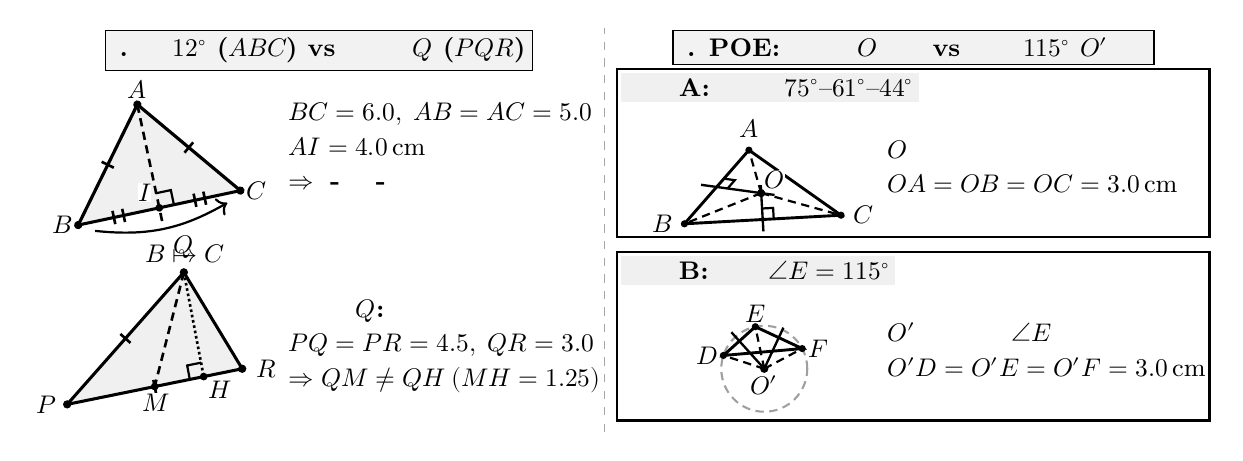
\begin{tikzpicture}[x=0.78cm, y=0.78cm, every node/.style={font=\linespread{1.0}\fontsize{9.2pt}{12.5pt}\selectfont, text=black}]
  \draw[line width=0.6pt, dashed, gray!70] (9.15, 0.05) -- (9.15, 6.62);
  \node[anchor=north, fill=headgray, draw=black, line width=0.5pt, inner sep=2.6pt] at (4.50, 6.60) {\textbf{ក. បត់ $12^\circ$ \en{($ABC$)} \en{vs} កំពូលខុស $Q$ \en{($PQR$)}}};
  \node[anchor=north, fill=headgray, draw=black, line width=0.5pt, inner sep=2.6pt] at (14.18, 6.60) {\textbf{ខ. \en{POE}: មុំស្រួច $O$ ក្នុង \en{vs} មុំទាល $115^\circ$ $O'$ ក្រៅ}};

  % Left top: Tilted 12 deg ABC (BC=6.0, AB=AC=5.0, AI=4.0)
  \begin{scope}[shift={(1.90, 3.70)}, rotate=12]
    \coordinate (B) at (-1.35, 0);
    \coordinate (C) at (1.35, 0);
    \coordinate (I) at (0, 0);
    \coordinate (A) at (0, 1.72);
    \fill[panelgray] (A) -- (B) -- (C) -- cycle;
    \draw[black, line width=1.15pt, tk1] (A) -- (B);
    \draw[black, line width=1.15pt, tk1] (A) -- (C);
    \draw[black, line width=1.1pt, tk2] (B) -- (I);
    \draw[black, line width=1.1pt, tk2] (I) -- (C);
    \draw[black, densely dashed, line width=0.95pt] (0, -0.22) -- (0, 1.95);
    \rightanglemark[0.19]{(I)}{(C)}{(A)}
    \draw[black, line width=0.8pt, ->, bend right=18] (-1.10, -0.15) to (1.10, -0.15);
    \node[fill=white, inner sep=0.5pt] at (0.0, -0.76) {បត់ \en{$B\mapsto C$}};
    \fill[black] (A) circle (1.5pt) node[above=1.5pt, fill=white, inner sep=0.5pt] {\en{$A$}};
    \fill[black] (B) circle (1.5pt) node[left=1.5pt, fill=white, inner sep=0.5pt] {\en{$B$}};
    \fill[black] (C) circle (1.5pt) node[right=1.5pt, fill=white, inner sep=0.5pt] {\en{$C$}};
    \fill[black] (I) circle (1.4pt) node[above left=2.5pt, xshift=-1pt, fill=white, inner sep=0.4pt] {\en{$I$}};
  \end{scope}
  \node[anchor=west, align=left] at (3.85, 4.70) {\en{$BC=6.0,\; AB=AC=5.0$}\\ \en{$AI=4.0\unit{cm}$}\\ $\Rightarrow$ \textbf{៤-ក្នុង-១}};

  % Left bottom: Wrong-Apex PQR (PQ=PR=4.5, QR=3.0) from base vertex Q
  \begin{scope}[shift={(0.40, 0.50)}]
    \coordinate (P) at (0.0, 0.0);
    \coordinate (R) at (2.85, 0.58);
    \coordinate (M) at ($(P)!0.50!(R)$);
    \coordinate (H) at ($(P)!0.78!(R)$);
    \coordinate (Q) at (1.90, 2.15);
    \fill[panelgray] (P) -- (Q) -- (R) -- cycle;
    \draw[black, line width=1.1pt, tk1] (P) -- (Q);
    \draw[black, line width=1.1pt, tk1] (P) -- (R);
    \draw[black, line width=1.1pt] (Q) -- (R);
    \draw[black, densely dashed, line width=0.95pt] (Q) -- (M);
    \draw[black, densely dotted, line width=0.95pt] (Q) -- (H);
    \rightanglemark[0.18]{(H)}{(P)}{(Q)}
    \fill[black] (P) circle (1.5pt) node[left=1.5pt] {\en{$P$}};
    \fill[black] (Q) circle (1.5pt) node[above=1.5pt] {\en{$Q$}};
    \fill[black] (R) circle (1.5pt) node[right=1.5pt] {\en{$R$}};
    \fill[black] (M) circle (1.4pt) node[below=2pt, fill=white, inner sep=0.4pt] {\en{$M$}};
    \fill[black] (H) circle (1.4pt) node[below right=1.5pt, fill=white, inner sep=0.4pt] {\en{$H$}};
  \end{scope}
  \node[anchor=west, align=left] at (3.85, 1.45) {\textbf{កំពូលខុស $Q$:}\\ \en{$PQ=PR=4.5,\; QR=3.0$}\\ \en{$\Rightarrow QM\neq QH\;(MH=1.25)$}};

  % Right top: POE Panel A (Acute 75-61-44, O inside)
  \begin{scope}[shift={(9.35, 3.22)}]
    \draw[black, line width=0.85pt] (0, 0) rectangle (9.65, 2.74);
    \node[anchor=north west, fill=panelgray, inner sep=1.8pt] at (0.06, 2.68) {\textbf{ផ្ទាំង \en{A}:} មុំស្រួច \en{$75^\circ\text{--}61^\circ\text{--}44^\circ$}};
    \coordinate (Oa) at (2.35, 0.72);
    \coordinate (Aa) at (2.15, 1.42);
    \coordinate (Ba) at (1.10, 0.22);
    \coordinate (Ca) at (3.65, 0.36);
    \coordinate (La) at ($(Aa)!0.5!(Ba)$);
    \coordinate (Ma) at ($(Ba)!0.5!(Ca)$);
    \draw[black, line width=1.05pt] (Aa) -- (Ba) -- (Ca) -- cycle;
    \draw[black, line width=0.85pt] ($(Oa)!-0.30!(La)$) -- ($(Oa)!1.35!(La)$);
    \draw[black, line width=0.85pt] ($(Oa)!-0.30!(Ma)$) -- ($(Oa)!1.45!(Ma)$);
    \rightanglemark[0.14]{(La)}{(Oa)}{(Aa)}
    \rightanglemark[0.14]{(Ma)}{(Oa)}{(Ca)}
    \draw[black, densely dashed, line width=0.8pt] (Oa) -- (Aa) (Oa) -- (Ba) (Oa) -- (Ca);
    \fill[black] (Aa) circle (1.3pt) node[above=1pt] {\en{$A$}};
    \fill[black] (Ba) circle (1.3pt) node[left=1pt] {\en{$B$}};
    \fill[black] (Ca) circle (1.3pt) node[right=1pt] {\en{$C$}};
    \fill[black] (Oa) circle (1.5pt) node[above right=1pt, fill=white, inner sep=0.4pt] {\en{$O$}};
    \node[anchor=west, align=left] at (4.25, 1.15) {$O$ នៅ\textbf{ខាងក្នុង}\\ \en{$OA=OB=OC=3.0\unit{cm}$}};
  \end{scope}

  % Right bottom: POE Panel B (Obtuse 115 deg, O' outside, circle)
  \begin{scope}[shift={(9.35, 0.24)}]
    \draw[black, line width=0.85pt] (0, 0) rectangle (9.65, 2.74);
    \node[anchor=north west, fill=panelgray, inner sep=1.8pt] at (0.06, 2.68) {\textbf{ផ្ទាំង \en{B}:} មុំទាល \en{$\ang{E}=115^\circ$}};
    \coordinate (Op) at (2.40, 0.84);
    \coordinate (Dp) at ($(Op)+(162:0.70)$);
    \coordinate (Ep) at ($(Op)+(102:0.70)$);
    \coordinate (Fp) at ($(Op)+(28:0.70)$);
    \coordinate (K1) at ($(Dp)!0.5!(Ep)$);
    \coordinate (K2) at ($(Ep)!0.5!(Fp)$);
    \draw[gray!75, densely dashed, line width=0.75pt] (Op) circle (0.70);
    \draw[black, line width=1.05pt] (Dp) -- (Ep) -- (Fp) -- cycle;
    \draw[black, line width=0.85pt] (Op) -- ($(Op)!1.32!(K1)$);
    \draw[black, line width=0.85pt] (Op) -- ($(Op)!1.32!(K2)$);
    \draw[black, densely dashed, line width=0.8pt] (Op) -- (Dp) (Op) -- (Ep) (Op) -- (Fp);
    \fill[black] (Dp) circle (1.3pt) node[left=1.5pt, fill=white, inner sep=0.4pt] {\en{$D$}};
    \fill[black] (Ep) circle (1.3pt) node[above=1pt, fill=white, inner sep=0.4pt] {\en{$E$}};
    \fill[black] (Fp) circle (1.3pt) node[right=1.5pt, fill=white, inner sep=0.4pt] {\en{$F$}};
    \fill[black] (Op) circle (1.5pt) node[below=2pt, fill=white, inner sep=0.4pt] {\en{$O'$}};
    \node[anchor=west, align=left] at (4.25, 1.15) {$O'$ នៅ\textbf{ខាងក្រៅ}ឈម $\ang{E}$\\ \en{$O'D=O'E=O'F=3.0\unit{cm}$}};
  \end{scope}
\end{tikzpicture}\par
\vspace{2pt}
{\fontsize{9.6pt}{13.0pt}\selectfont\textbf{រូបទី ១៖} ការបត់ \en{1:1} ទ្រេត $12^\circ$ ធៀបនឹងរូបកំពូលខុស $Q$ និង \en{POE} មុំស្រួច $O$ ក្នុងទល់នឹងមុំទាល $115^\circ$ $O'$ ក្រៅ \en{(Olson, 1975; Coad, 2006; Catman-Aksoy \& Isiksal-Bostan, 2024; Yıldız et al., 2010; Bento et al., 2018)}។}
\end{tcolorbox}

% --- រូបទី ២ ---
\begin{tcolorbox}[enhanced, breakable, sharp corners, colback=white, colframe=black, boxrule=0.8pt, top=4pt, bottom=3pt, left=4pt, right=4pt, before skip=2pt, after skip=3pt]
\centering
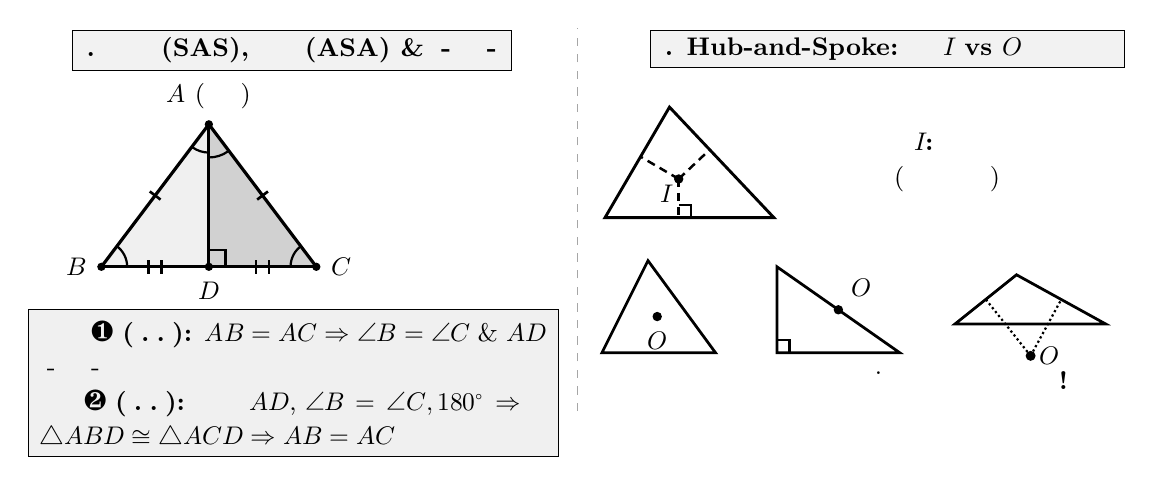
\begin{tikzpicture}[x=0.78cm, y=0.78cm, every node/.style={font=\linespread{1.0}\fontsize{9.2pt}{12.5pt}\selectfont, text=black}]
  \draw[line width=0.6pt, dashed, gray!70] (9.10, 0.05) -- (9.10, 6.28);
  \node[anchor=north, fill=headgray, draw=black, line width=0.5pt, inner sep=2.6pt] at (4.45, 6.26) {\textbf{ក. ផ្ទាល់ \en{(SAS)}, ច្រាស \en{(ASA)} \& ៤-ក្នុង-១}};
  \node[anchor=north, fill=headgray, draw=black, line width=0.5pt, inner sep=2.6pt] at (14.15, 6.26) {\textbf{ខ. \en{Hub-and-Spoke}: ញែក $I$ \en{vs} $O$ តាមប្រភេទមុំ}};

  % Left: Direct & Converse ASA + 4-in-1 from apex A
  \coordinate (B2) at (1.35, 2.40);
  \coordinate (C2) at (4.85, 2.40);
  \coordinate (D2) at (3.10, 2.40);
  \coordinate (A2) at (3.10, 4.72);
  \fill[panelgray] (A2) -- (B2) -- (D2) -- cycle;
  \fill[midgray] (A2) -- (D2) -- (C2) -- cycle;
  \draw[black, line width=1.15pt, tk1] (A2) -- (B2);
  \draw[black, line width=1.15pt, tk1] (A2) -- (C2);
  \draw[black, line width=1.1pt, tk2] (B2) -- (D2);
  \draw[black, line width=1.1pt, tk2] (D2) -- (C2);
  \draw[black, line width=1.1pt] (A2) -- (D2);
  \rightanglemark[0.21]{(D2)}{(C2)}{(A2)}
  \draw[ang1] ($(B2)+(0:0.42)$) arc (0:55:0.42);
  \draw[ang1] ($(C2)+(180:0.42)$) arc (180:125:0.42);
  \draw[ang1] ($(A2)+(-125:0.46)$) arc (-125:-90:0.46);
  \draw[ang1] ($(A2)+(-90:0.54)$) arc (-90:-55:0.54);
  \fill[black] (A2) circle (1.5pt) node[above=2pt] {\en{$A$} (កំពូល)};
  \fill[black] (B2) circle (1.5pt) node[left=2pt] {\en{$B$}};
  \fill[black] (C2) circle (1.5pt) node[right=2pt] {\en{$C$}};
  \fill[black] (D2) circle (1.5pt) node[below=2pt] {\en{$D$}};
  \node[anchor=north west, draw=black, fill=panelgray, line width=0.65pt, inner sep=4pt, align=left, text width=6.45cm] at (0.15, 1.72) {%
    \textbf{ផ្ទាល់ \cnum{1} (\textbf{ជ.ម.ជ}):} $AB=AC \Rightarrow \ang{B}=\ang{C}$ \& $AD$ ៤-ក្នុង-១។\\
    \textbf{ច្រាស \cnum{2} (\textbf{ម.ជ.ម}):} ពុះមុំ $AD$, $\ang{B}=\ang{C}, 180^\circ \Rightarrow \tri{ABD}\cg\tri{ACD} \Rightarrow AB=AC$។};

  % Right top: I (incenter, inside always) vs O (circumcenter)
  \begin{scope}[shift={(9.55, 3.05)}]
    \coordinate (Ai) at (1.05, 1.95);
    \coordinate (Bi) at (0.0, 0.15);
    \coordinate (Ci) at (2.75, 0.15);
    \coordinate (Ii) at (1.20, 0.78);
    \draw[black, line width=1.05pt] (Ai) -- (Bi) -- (Ci) -- cycle;
    \draw[black, densely dashed, line width=0.9pt] (Ii) -- (1.20, 0.15);
    \draw[black, densely dashed, line width=0.9pt] (Ii) -- ($(Ai)!(Ii)!(Bi)$);
    \draw[black, densely dashed, line width=0.9pt] (Ii) -- ($(Ai)!(Ii)!(Ci)$);
    \rightanglemark[0.16]{(1.20,0.15)}{(Ci)}{(Ii)}
    \fill[black] (Ii) circle (1.7pt) node[below left=2.5pt, fill=white, inner sep=0.4pt] {\en{$I$}};
    \node[anchor=west, align=left] at (3.20, 1.05) {\textbf{ប្រសព្វពុះមុំ $I$:} ស្មើចម្ងាយ\\កែង\textbf{ជ្រុង ៣} (ក្នុងជានិច្ច)};
  \end{scope}

  % Right bottom: 3 positions of O (Acute inside, Right mid-hyp, Obtuse outside)
  \begin{scope}[shift={(9.50, 0.55)}]
    % Acute
    \draw[black, line width=1.0pt] (0.0, 0.45) -- (1.85, 0.45) -- (0.75, 1.95) -- cycle;
    \fill[black] (0.90, 1.04) circle (1.7pt) node[below=2pt] {\en{$O$}};
    \node[anchor=north] at (0.92, 0.30) {ស្រួច៖ ក្នុង};
    % Right
    \coordinate (r1) at (2.85, 0.45);
    \coordinate (r2) at (4.85, 0.45);
    \coordinate (r3) at (2.85, 1.85);
    \draw[black, line width=1.0pt] (r1) -- (r2) -- (r3) -- cycle;
    \rightanglemark[0.16]{(r1)}{(r2)}{(r3)}
    \fill[black] (3.85, 1.15) circle (1.7pt) node[above right=1.5pt] {\en{$O$}};
    \node[anchor=north] at (3.85, 0.30) {កែង៖ អ៊ីប៉ូ.};
    % Obtuse
    \coordinate (o1) at (5.75, 0.92);
    \coordinate (o2) at (6.75, 1.72);
    \coordinate (o3) at (8.20, 0.92);
    \draw[black, line width=1.0pt] (o1) -- (o2) -- (o3) -- cycle;
    \fill[black] (6.98, 0.40) circle (1.8pt) node[right=2.5pt, fill=white, inner sep=0.4pt] {\en{$O$}};
    \draw[black, densely dotted, line width=0.8pt] (6.98, 0.40) -- (6.25, 1.32) (6.98, 0.40) -- (7.48, 1.32);
    \node[anchor=north] at (6.98, 0.30) {ទាល៖ \textbf{ក្រៅ!}};
  \end{scope}
\end{tikzpicture}\par
\vspace{2pt}
{\fontsize{9.6pt}{13.0pt}\selectfont\textbf{រូបទី ២៖} ទ្រឹស្ដីបទផ្ទាល់-ច្រាស (\en{SAS/ASA}) និង \en{Hub-and-Spoke} ញែក $I$ ពី $O$ តាមមុំត្រីកោណ \en{(Winer \& Battista, 2022; Xu et al., 2026; Demiray et al., 2023; Yıldız et al., 2010)}។}
\end{tcolorbox}

% --- រូបទី ៣ ---
\begin{tcolorbox}[enhanced, breakable, sharp corners, colback=white, colframe=black, boxrule=0.8pt, top=4pt, bottom=3pt, left=4pt, right=4pt, before skip=2pt, after skip=3pt]
\centering
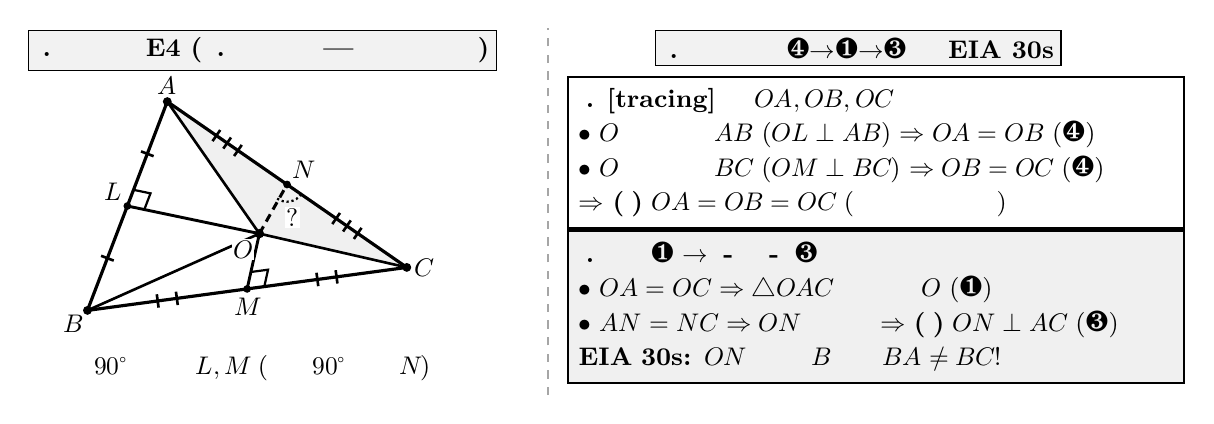
\begin{tikzpicture}[x=0.78cm, y=0.78cm, every node/.style={font=\linespread{1.0}\fontsize{9.2pt}{12.5pt}\selectfont, text=black}]
  \draw[line width=0.6pt, dashed, gray!70] (9.10, 0.05) -- (9.10, 6.02);
  \node[anchor=north, fill=headgray, draw=black, line width=0.5pt, inner sep=2.6pt] at (4.45, 6.00) {\textbf{ក. លំហាត់គំរូ \en{E4} (ទំ.១៥៧ កែតម្រូវ — មុំស្រួចមិនសមបាទ)}};
  \node[anchor=north, fill=headgray, draw=black, line width=0.5pt, inner sep=2.6pt] at (14.15, 6.00) {\textbf{ខ. ច្រវាក់ស្រាយ \cnum{4}$\to$\cnum{1}$\to$\cnum{3} និង \en{EIA 30s}}};

  % Left: Corrected Book p.157 figure (visibly scalene acute ABC, 90° ONLY at L & M, dashed ON + ?, non-collinear A-O-M & B-O-N)
  \begin{scope}[shift={(0.75, 0.38)}]
    \coordinate (O) at (3.65, 2.30);
    \coordinate (A) at (2.15, 4.45);
    \coordinate (B) at (0.85, 1.05);
    \coordinate (C) at (6.05, 1.75);
    \coordinate (L) at ($(A)!0.5!(B)$);
    \coordinate (M) at ($(B)!0.5!(C)$);
    \coordinate (N) at ($(A)!0.5!(C)$);
    \fill[panelgray] (O) -- (A) -- (C) -- cycle;
    \draw[black, line width=1.15pt, tk1] (A) -- (L);
    \draw[black, line width=1.15pt, tk1] (L) -- (B);
    \draw[black, line width=1.15pt, tk2] (B) -- (M);
    \draw[black, line width=1.15pt, tk2] (M) -- (C);
    \draw[black, line width=1.15pt, tk3] (A) -- (N);
    \draw[black, line width=1.15pt, tk3] (N) -- (C);
    \draw[black, line width=0.95pt] (O) -- (A) (O) -- (B) (O) -- (C);
    \draw[black, line width=1.05pt] (O) -- (L) (O) -- (M);
    \rightanglemark[0.22]{(L)}{(A)}{(O)}
    \rightanglemark[0.22]{(M)}{(C)}{(O)}
    \draw[black, densely dashed, line width=1.1pt] (O) -- (N);
    \draw[black, densely dotted, line width=0.8pt] ($(N)+(-125:0.28)$) arc (-125:-35:0.28);
    \node[fill=white, inner sep=0.5pt] at ($(N)+(-80:0.54)$) {\en{$?$}};
    \fill[black] (A) circle (1.6pt) node[above=2pt, fill=white, inner sep=0.5pt] {\en{$A$}};
    \fill[black] (B) circle (1.6pt) node[below left=1.5pt, fill=white, inner sep=0.5pt] {\en{$B$}};
    \fill[black] (C) circle (1.6pt) node[right=2pt, fill=white, inner sep=0.5pt] {\en{$C$}};
    \fill[black] (L) circle (1.4pt) node[above left=2pt, fill=white, inner sep=0.5pt] {\en{$L$}};
    \fill[black] (M) circle (1.4pt) node[below=2.5pt, fill=white, inner sep=0.5pt] {\en{$M$}};
    \fill[black] (N) circle (1.4pt) node[above right=2pt, fill=white, inner sep=0.5pt] {\en{$N$}};
    \fill[black] (O) circle (1.7pt) node[below left=2.5pt, fill=white, inner sep=0.5pt] {\en{$O$}};
    \node[anchor=south] at (3.45, -0.25) {កែង \en{$90^\circ$} តែត្រង់ \en{$L, M$} (គ្មាន \en{$90^\circ$} ត្រង់ \en{$N$})};
  \end{scope}

  % Right: Proof Chain & EIA 30s Callout
  \node[anchor=north west, draw=black, fill=white, line width=0.8pt, inner sep=4pt, align=left, text width=7.55cm] at (9.40, 5.25) {%
    \textbf{១. \en{[tracing]} តាម $OA, OB, OC$៖}\\
    $\bullet$ $O$ លើមេដ្យាទ័រ $AB$ ($OL\perp AB$) $\Rightarrow OA=OB$ (\cnum{4})\\
    $\bullet$ $O$ លើមេដ្យាទ័រ $BC$ ($OM\perp BC$) $\Rightarrow OB=OC$ (\cnum{4})\\
    $\Rightarrow$ \textbf{(ក)} $OA = OB = OC$ (ផ្ចិតរង្វង់ចារឹកក្រៅ)};
  \node[anchor=north west, draw=black, fill=panelgray, line width=0.8pt, inner sep=4pt, align=left, text width=7.55cm] at (9.40, 2.75) {%
    \textbf{២. សមបាទ \cnum{1} $\to$ ៤-ក្នុង-១ \cnum{3}៖}\\
    $\bullet$ $OA=OC \Rightarrow \tri{OAC}$ សមបាទកំពូល $O$ (\cnum{1})\\
    $\bullet$ $AN=NC \Rightarrow ON$ ជាមេដ្យាន $\Rightarrow$ \textbf{(ខ)} $ON\perp AC$ (\cnum{3})\\
    \textbf{EIA 30s:} $ON$ មិនកាត់ $B$ ព្រោះ $BA\neq BC$!};
\end{tikzpicture}\par
\vspace{2pt}
{\fontsize{9.6pt}{13.0pt}\selectfont\textbf{រូបទី ៣៖} លំហាត់គំរូ \en{E4} (ទំ.១៥៧ កែតម្រូវ គ្មាន $90^\circ$ ត្រង់ $N$ និង $A$-$O$-$M$ មិនត្រង់ជួរ) និងច្រវាក់ហេតុផល \en{(Yeo \& Tzeng, 2019; Miyazaki et al., 2019; Yıldız et al., 2010)}។}
\end{tcolorbox}

% --- រូបទី ៤ ---
\begin{tcolorbox}[enhanced, breakable, sharp corners, colback=white, colframe=black, boxrule=0.8pt, top=4pt, bottom=3pt, left=4pt, right=4pt, before skip=2pt, after skip=3pt]
\centering
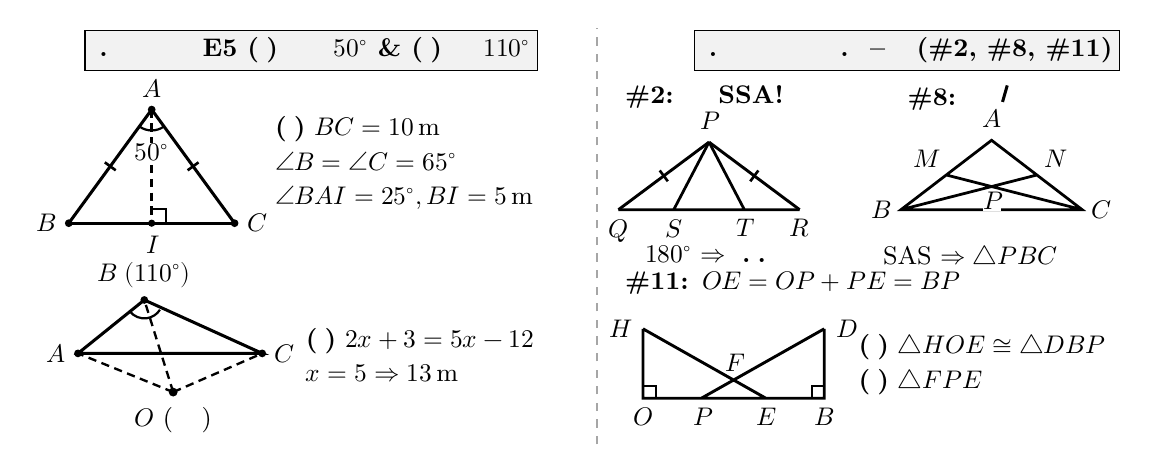
\begin{tikzpicture}[x=0.78cm, y=0.78cm, every node/.style={font=\linespread{1.0}\fontsize{9.2pt}{12.5pt}\selectfont, text=black}]
  \draw[line width=0.6pt, dashed, gray!70] (9.10, 0.05) -- (9.10, 6.82);
  \node[anchor=north, fill=headgray, draw=black, line width=0.5pt, inner sep=2.6pt] at (4.45, 6.80) {\textbf{ក. ប្រតិបត្តិ \en{E5} (ក) ហោជាង $50^\circ$ \& (ខ) ប៉ម $110^\circ$}};
  \node[anchor=north, fill=headgray, draw=black, line width=0.5pt, inner sep=2.6pt] at (14.15, 6.80) {\textbf{ខ. កិច្ចការផ្ទះ ទំ.១៦៤--១៦៥ (\en{\#2, \#8, \#11})}};

  % Left top: E5 (a) Gable ABC (A=50, BC=10 m)
  \begin{scope}[shift={(0.50, 3.65)}]
    \coordinate (Bg) at (0.0, 0.0);
    \coordinate (Cg) at (2.70, 0.0);
    \coordinate (Ig) at (1.35, 0.0);
    \coordinate (Ag) at (1.35, 1.85);
    \draw[black, line width=1.1pt, tk1] (Ag) -- (Bg);
    \draw[black, line width=1.1pt, tk1] (Ag) -- (Cg);
    \draw[black, line width=1.1pt] (Bg) -- (Cg);
    \draw[black, densely dashed, line width=0.95pt] (Ag) -- (Ig);
    \rightanglemark[0.18]{(Ig)}{(Cg)}{(Ag)}
    \draw[ang1] ($(Ag)+(-126:0.34)$) arc (-126:-54:0.34);
    \node[fill=white, inner sep=0.4pt] at (1.35, 1.15) {\en{$50^\circ$}};
    \fill[black] (Ag) circle (1.4pt) node[above=1pt] {\en{$A$}};
    \fill[black] (Bg) circle (1.4pt) node[left=1pt] {\en{$B$}};
    \fill[black] (Cg) circle (1.4pt) node[right=1pt] {\en{$C$}};
    \fill[black] (Ig) circle (1.3pt) node[below=1pt] {\en{$I$}};
    \node[anchor=west, align=left] at (3.20, 0.98) {\textbf{(ក)} $BC=10\unit{m}$\\ $\ang{B}=\ang{C}=65^\circ$\\ $\ang{BAI}=25^\circ, BI=5\unit{m}$};
  \end{scope}

  % Left bottom: E5 (b) Obtuse 110 deg tower O outside
  \begin{scope}[shift={(0.45, 0.45)}]
    \coordinate (Ot) at (1.75, 0.45);
    \coordinate (At) at (0.20, 1.08);
    \coordinate (Bt) at (1.28, 1.95);
    \coordinate (Ct) at (3.20, 1.08);
    \draw[black, line width=1.1pt] (At) -- (Bt) -- (Ct) -- cycle;
    \draw[black, densely dashed, line width=0.85pt] (Ot) -- (At) (Ot) -- (Bt) (Ot) -- (Ct);
    \draw[ang1] ($(Bt)+(-142:0.30)$) arc (-142:-32:0.30);
    \fill[black] (At) circle (1.4pt) node[left=1pt] {\en{$A$}};
    \fill[black] (Bt) circle (1.4pt) node[above=1pt] {\en{$B\;(110^\circ)$}};
    \fill[black] (Ct) circle (1.4pt) node[right=1pt] {\en{$C$}};
    \fill[black] (Ot) circle (1.6pt) node[below=2pt] {\en{$O$} (ក្រៅ)};
    \node[anchor=west, align=left] at (3.75, 1.05) {\textbf{(ខ)} $2x+3=5x-12$\\ \en{$x=5 \Rightarrow 13\unit{m}$}};
  \end{scope}

  % Right top-left: HW #2 (SSA trap)
  \begin{scope}[shift={(9.45, 3.72)}]
    \node[anchor=west] at (-0.05, 1.98) {\textbf{\en{\#2:} ហាម \en{SSA}!}};
    \coordinate (q2) at (0.0, 0.15); \coordinate (s2) at (0.90, 0.15);
    \coordinate (t2) at (2.05, 0.15); \coordinate (r2) at (2.95, 0.15);
    \coordinate (p2) at (1.475, 1.25);
    \draw[black, line width=1.05pt, tk1] (p2) -- (q2);
    \draw[black, line width=1.05pt, tk1] (p2) -- (r2);
    \draw[black, line width=1.0pt] (q2) -- (r2) (p2) -- (s2) (p2) -- (t2);
    \node[above=1pt] at (p2) {\en{$P$}}; \node[below=0pt] at (q2) {\en{$Q$}};
    \node[below=0pt] at (s2) {\en{$S$}}; \node[below=0pt] at (t2) {\en{$T$}}; \node[below=0pt] at (r2) {\en{$R$}};
    \node[anchor=north] at (1.475, -0.28) {\en{$180^\circ$} $\Rightarrow$ \textbf{ម.ជ.ម}};
  \end{scope}

  % Right top-right: HW #8 (zero-tick -> SAS -> Converse)
  \begin{scope}[shift={(14.05, 3.72)}]
    \node[anchor=west] at (-0.05, 1.98) {\textbf{\en{\#8:} គូស \tickone{} លើរូប}};
    \coordinate (b8) at (0.0, 0.15); \coordinate (c8) at (2.95, 0.15); \coordinate (a8) at (1.475, 1.28);
    \coordinate (m8) at ($(a8)!0.5!(b8)$); \coordinate (n8) at ($(a8)!0.5!(c8)$);
    \coordinate (p8) at (1.475, 0.52);
    \draw[black, line width=1.0pt] (a8) -- (b8) -- (c8) -- cycle (b8) -- (n8) (c8) -- (m8);
    \node[above=1pt] at (a8) {\en{$A$}}; \node[left=0pt] at (b8) {\en{$B$}}; \node[right=0pt] at (c8) {\en{$C$}};
    \node[above left=-1pt] at (m8) {\en{$M$}}; \node[above right=-1pt] at (n8) {\en{$N$}};
    \node[below=1.5pt, fill=white, inner sep=0.3pt] at (p8) {\en{$P$}};
    \node[anchor=north] at (1.475, -0.28) {\en{SAS} $\Rightarrow \tri{PBC}$ សមបាទ};
  \end{scope}

  % Right bottom: HW #11 (HO perp OB, DB perp OB, OE=BP -> SAS -> FPE isosceles)
  \begin{scope}[shift={(9.85, 0.45)}]
    \node[anchor=west] at (-0.45, 2.22) {\textbf{\en{\#11:} $OE=OP+PE=BP$}};
    \coordinate (o11) at (0.0, 0.35); \coordinate (p11) at (0.95, 0.35);
    \coordinate (e11) at (2.00, 0.35); \coordinate (b11) at (2.95, 0.35);
    \coordinate (h11) at (0.0, 1.48); \coordinate (d11) at (2.95, 1.48);
    \coordinate (f11) at (1.475, 0.68);
    \draw[black, line width=1.05pt] (h11) -- (o11) -- (b11) -- (d11) (h11) -- (e11) (d11) -- (p11);
    \rightanglemark[0.16]{(o11)}{(e11)}{(h11)}
    \rightanglemark[0.16]{(b11)}{(p11)}{(d11)}
    \node[left=1pt] at (h11) {\en{$H$}}; \node[right=1pt] at (d11) {\en{$D$}};
    \node[below=0pt] at (o11) {\en{$O$}}; \node[below=0pt] at (p11) {\en{$P$}};
    \node[below=0pt] at (e11) {\en{$E$}}; \node[below=0pt] at (b11) {\en{$B$}};
    \node[above=2pt, fill=white, inner sep=0.3pt] at (f11) {\en{$F$}};
    \node[anchor=west, align=left] at (3.35, 0.90) {\textbf{(ក)} $\tri{HOE}\cg\tri{DBP}$\\ \textbf{(ខ)} $\tri{FPE}$ សមបាទ};
  \end{scope}
\end{tikzpicture}\par
\vspace{2pt}
{\fontsize{9.6pt}{13.0pt}\selectfont\textbf{រូបទី ៤៖} លំហាត់ប្រតិបត្តិ \en{E5} (ហោជាង $50^\circ$ \& ប៉មទឹក $110^\circ$) និងគំនូសវិភាគកិច្ចការផ្ទះ \en{\#2, \#8, \#11} ទំ.១៦៤--១៦៥ \en{(Milin Šipuš et al., 2022; Scristia et al., 2022; Biber, 2020)}។}
\end{tcolorbox}

% ============================================================================
% ផ្នែកទី ៦៖ មគ្គុទ្ទេសក៍រៀបចំ និងប្រើប្រាស់សម្ភារៈបោះពុម្ព (Pages 1--6) & ចម្លើយពេញលេញ
% ============================================================================
\secbanner{ផ្នែកទី ៦៖ មគ្គុទ្ទេសក៍រៀបចំ និងប្រើប្រាស់សម្ភារៈបោះពុម្ព \enbf{(Pages 1--6)}}{Section 6: Printing Calibration (Actual Size 100\%), Cut-Out Preparation \& Complete Master Answer Keys}

\subsec{៦\enbf{.}១ ស្តង់ដារបោះពុម្ព \enbf{Actual Size 100\%} និងលំដាប់ចែកសន្លឹកកិច្ចការ}

\begin{enumerate}[leftmargin=0.65cm, itemsep=2.5pt]
  \item \textbf{ការកំណត់បោះពុម្ព \en{1:1} ដាច់ខាត (ទំព័រ ១)៖} បោះពុម្ពឯកសារ \en{Printable\_Materials\_ISO.pdf} ដោយជ្រើស \textbf{\en{Scale: Actual Size 100\%}} (\emph{ហាមប្រើ} \en{Fit to Page / Shrink to Fit}) ហើយវាស់ផ្ទៀងបន្ទះក្រិត \textbf{\en{5.0 cm}} នៅខាងស្ដាំផ្នែកខាងលើទំព័រ ១ ដើម្បីធានាថា $\tri{ABC}$ ($BC=6.0\unit{cm}, AB=AC=5.0\unit{cm}, AI=4.0\unit{cm}$), បន្ទះកំពូលខុស $\tri{PQR}$ ($4.5, 4.5, 3.0\unit{cm}$), និង \en{POE Panel A--B} កាំ $3.00\unit{cm}$ មានខ្នាត \en{1:1} ពិតប្រាកដ។
  \item \textbf{ទម្រង់សន្សំក្រដាស ស-ខ្មៅ (ទំព័រ ២--៦)៖} ទំព័រ ២ (កាត \en{E4}) និងទំព័រ ៣ (សន្លឹក \en{E5} ៣ តួនាទី) ជាទម្រង់ \en{2-up} (២ ប័ណ្ណ/សន្លឹកក្នុង ១ ទំព័រ \en{A4}), ទំព័រ ៤ (ផ្ទាំងយោងប្រចាំថ្នាក់ និងធនាគារ \cnum{1}--\cnum{5}) គួរបោះពុម្ពលើក្រដាសរឹង \en{180 gsm} បិទលើក្ដារខៀន, ទំព័រ ៥ ជាកាតត្រួតពិនិត្យ \en{A--D} \en{4-up} + ចម្លើយគ្រូ, និងទំព័រ ៦ ជាប័ណ្ណកិច្ចការផ្ទះ \en{4-up}។
  \item \textbf{ឧបករណ៍តុក្រុម ៣ នាក់៖} កន្ត្រៃ ១, បន្ទាត់ក្រិត \en{cm/mm} ១, រ៉ាព័រទ័រ ១, និងដែកឈាន ១ ក្នុងមួយក្រុម។ ចែកទំព័រ ១ ផ្កាប់លើតុនៅនាទី ០០', ទំព័រ ២ នៅនាទី ២៨', ទំព័រ ៣ នៅនាទី ៣៨', បង្ហាញទំព័រ ៥ នៅនាទី ៤៤.៥', និងចែកទំព័រ ៦ នៅនាទី ៤៨'។
\end{enumerate}

\subsec{៦\enbf{.}២ ចម្លើយគំរូពេញលេញសម្រាប់គ្រប់សន្លឹកកិច្ចការ និងលំហាត់ \enbf{(Pages 1--6 \& HW)}}

\begingroup
\linespread{1.05}\fontsize{10.5pt}{15.5pt}\selectfont
\begin{longtable}{|L{2.95cm}|L{13.90cm}|}
\hline
\rowcolor{headgray}
\multicolumn{1}{|C{2.95cm}|}{\tblhead{សន្លឹក \enbf{/} លំហាត់}} &
\multicolumn{1}{C{13.90cm}|}{\tblhead{ចម្លើយគំរូផ្លូវការ និងពិន្ទុត្រួតពិនិត្យ \enbf{(Master Key)}}} \\
\hline
\endfirsthead
\hline
\rowcolor{headgray}
\multicolumn{1}{|C{2.95cm}|}{\tblhead{សន្លឹក \enbf{/} លំហាត់}} &
\multicolumn{1}{C{13.90cm}|}{\tblhead{ចម្លើយគំរូផ្លូវការ និងពិន្ទុត្រួតពិនិត្យ \enbf{(Master Key)}}} \\
\hline
\endhead
\hline
\endfoot
\hline
\endlastfoot
\textbf{ទំព័រ ១ (\en{E2})} \newline ស.១ \en{$\tri{ABC}$} &
\textbf{១. បត់ $\tri{ABC}$ ទ្រេត $12^\circ$ ($BC=6.0, AB=AC=5.0, AI=4.0\unit{cm}$):} បត់ $B\mapsto C$ តាម $(AI)$ បាន $IB=IC=\mathbf{3.0\unit{cm}}$, $\ang{AIB}=\mathbf{90^\circ}$, $\ang{B}=\ang{C}$, និង $\ang{BAI}=\ang{CAI}$ ($\Rightarrow (AI)$ ជា\textbf{បន្ទាត់រួម ៤-ក្នុង-១})។ \\
\hline
\textbf{ទំព័រ ១ (\en{E2})} \newline ស.១ \en{$\tri{PQR}$} &
\textbf{២. បន្ទះកំពូលខុស $\tri{PQR}$ ($PQ=PR=4.5, QR=3.0\unit{cm}$) ពីបាទ $Q$:} $QP=4.5\unit{cm}\neq QR=3.0\unit{cm}$; មេដ្យាន $QM$ ($PM=MR=\mathbf{2.25\unit{cm}}$, $\ang{QMR}\approx 66^\circ\neq 90^\circ$) $\neq$ កម្ពស់ $QH\perp PR$ ($PH=\mathbf{3.50\unit{cm}}, HR=\mathbf{1.00\unit{cm}}$; គម្លាត $MH=\mathbf{1.25\unit{cm}}$); បត់ $P\mapsto R$ មិនត្រួតគ្នាទេ។ \\
\hline
\textbf{ទំព័រ ១ (\en{E2})} \newline \en{POE Panel A} &
\textbf{ផ្ទាំង \en{A} ($\tri{ABC}$ មុំស្រួច $75^\circ, 61^\circ, 44^\circ$):} មេដ្យាទ័រ $d_1, d_2$ ប្រសព្វត្រង់ $O$ \textbf{ខាងក្នុង} $\tri{ABC}$ ហើយ $OA=OB=OC=\mathbf{3.0\unit{cm}}$។ \\
\hline
\textbf{ទំព័រ ១ (\en{E2})} \newline \en{POE Panel B} &
\textbf{ផ្ទាំង \en{B} ($\tri{DEF}$ មុំទាល $\ang{E}=115^\circ$):} បន្លាយមេដ្យាទ័រ $d'_1, d'_2$ ប្រសព្វត្រង់ $O'$ \textbf{ខាងក្រៅ} $\tri{DEF}$ (ឈម $\ang{E}=115^\circ$) តែរង្វង់ចារឹកក្រៅផ្ទៀង $O'D=O'E=O'F=\mathbf{3.00\unit{cm}}$ ស្មើគ្នា (ព្រោះ $O'$ ស្ថិតនៅលើមេដ្យាទ័រទាំងបី)។ \\
\hline
\textbf{ទំព័រ ២ (\en{E4})} \newline លំហាត់គំរូ (ក) &
\textbf{(ក) $OA=OB=OC$:} \en{[tracing]} តាម $OA, OB, OC$: $O$ លើមេដ្យាទ័រ $AB$ ($AL=LB, 90^\circ$) $\Rightarrow OA=OB$ (\cnum{4}); $O$ លើមេដ្យាទ័រ $BC$ ($BM=MC, 90^\circ$) $\Rightarrow OB=OC$ (\cnum{4}) $\Rightarrow \mathbf{OA=OB=OC}$។ \\
\hline
\textbf{ទំព័រ ២ (\en{E4})} \newline លំហាត់គំរូ (ខ) &
\textbf{(ខ) $ON\perp AC$:} \en{[tracing]} ជុំវិញ $\tri{OAC}$: ពី (ក) $OA=OC \Rightarrow \tri{OAC}$ សមបាទកំពូល $O$ (\cnum{1}); ដោយ $N$ កណ្ដាល $AC$ ($AN=NC$) នោះ $ON$ ជាមេដ្យានចេញពីកំពូល $O \Rightarrow \mathbf{ON\perp AC}$ ($90^\circ$, \cnum{3} ៤-ក្នុង-១)។ \newline
\textbf{\en{EIA 30s}:} $ON$ មិនកាត់ $B$ ព្រោះ $\tri{ABC}$ ជាត្រីកោណសាមញ្ញ ($BA\neq BC$)។ \\
\hline
\textbf{ទំព័រ ៣ (\en{E5})} \newline តួនាទី ១--២ (ក) &
\textbf{តួនាទី ១ (\en{Pause-Ask}):} គូស \tickone{} លើ $AB=AC$, $90^\circ$ ត្រង់ $I$ (ក), និងពិនិត្យ $O$ ក្រៅ $\tri{ABC}$ (ខ)។ \newline
\textbf{តួនាទី ២ (ក) ហោជាង:} $\tri{ABC}$ ($AB=AC, \ang{A}=50^\circ, AI\perp BC, BC=10\unit{m}$): តាម \cnum{1}, \cnum{5} $\Rightarrow \ang{B}=\ang{C}=\frac{180^\circ-50^\circ}{2}=\mathbf{65^\circ}$; តាម \cnum{3} $\Rightarrow \ang{BAI}=\frac{50^\circ}{2}=\mathbf{25^\circ}$, $BI=IC=\mathbf{5\unit{m}}$។ \\
\hline
\textbf{ទំព័រ ៣ (\en{E5})} \newline តួនាទី ២ (ខ) \& ៣ &
\textbf{តួនាទី ២ (ខ) ផ្លូវកោង:} $\ang{B}=110^\circ, OA=(2x+3)\unit{m}, OC=(5x-12)\unit{m}$: តាម \cnum{4} $\Rightarrow OA=OB=OC \Rightarrow 2x+3=5x-12 \Rightarrow 3x=15 \Rightarrow \mathbf{x=5} \Rightarrow OA=OB=OC=\mathbf{13\unit{m}}$។ \newline
\textbf{តួនាទី ៣ (\en{Pause-Review}):} ផ្ទៀង $2(5)+3=13\unit{m}, 5(5)-12=13\unit{m}$; ដោយ $\ang{B}=110^\circ>90^\circ \Rightarrow O$ នៅ\textbf{ខាងក្រៅ}ឈម $B$ តែស្មើចម្ងាយ $13\unit{m}$ ពីផ្ទះទាំង ៣។ \\
\hline
\textbf{ទំព័រ ៤} \newline ធនាគារ \cnum{1}--\cnum{3} &
\cnum{1} លក្ខណៈផ្ទាល់ត្រីកោណសមបាទ ($AB=AC\Rightarrow\ang{B}=\ang{C}$) $\vert$ \cnum{2} លក្ខណៈច្រាសត្រីកោណសមបាទ ($\ang{B}=\ang{C}\Rightarrow AB=AC$, \textbf{ម.ជ.ម}) $\vert$ \cnum{3} បន្ទាត់រួម ៤-ក្នុង-១ ចេញពីកំពូល (មេដ្យាទ័រ$\equiv$មេដ្យាន$\equiv$កម្ពស់$\equiv$ពុះមុំកំពូល)។ \\
\hline
\textbf{ទំព័រ ៤} \newline ធនាគារ \cnum{4}--\cnum{5} &
\cnum{4} ទ្រឹស្ដីបទមេដ្យាទ័រ \& ប្រសព្វ $O$ ($OA=OB=OC$) $\vert$ \cnum{5} លក្ខខណ្ឌត្រីកោណប៉ុនគ្នា (\textbf{ម.ជ.ម/ជ.ម.ជ/ជ.ជ.ជ/អ.ជ}, ហាម \en{SSA}!) និង $180^\circ$។ \\
\hline
\textbf{ទំព័រ ៥} \newline (កាត \en{A--B}) &
\textbf{កាត \en{A} (\ding{51} មេដៃឡើង):} $AB=AC, \ang{A}=40^\circ, BM=MC \Rightarrow AM$ ជា ៤-ក្នុង-១ (\cnum{3}): $AM\perp BC, \ang{BAM}=\mathbf{20^\circ}, \ang{B}=\ang{C}=\mathbf{70^\circ}$ (\cnum{1}, \cnum{5})។ \newline
\textbf{កាត \en{B} (\ding{55} ខ្វែងដៃ):} អន្ទាក់កំពូលខុស! $DE=DF=6\unit{cm}, EF=4\unit{cm}$ ($D$ ជាកំពូល មិនមែន $E$ ទេ) $\Rightarrow EK\not\perp DF$។ \\
\hline
\textbf{ទំព័រ ៥} \newline (កាត \en{C--D}) &
\textbf{កាត \en{C} (\ding{55} ខ្វែងដៃ):} ច្រឡំ $I$ នឹង $O$! ក្នុង $\tri{PQR}$ ($5,8,9$) ពុះមុំ $I$ ស្មើចម្ងាយកែងទៅ\textbf{ជ្រុង ៣} មិនមែន $IP=IQ=IR$ ទេ។ \newline
\textbf{កាត \en{D} (\ding{55} ខ្វែងដៃ):} អន្ទាក់មុំទាល! $\ang{Y}=120^\circ > 90^\circ \Rightarrow$ ប្រសព្វមេដ្យាទ័រ $O$ ស្ថិតនៅ\textbf{ខាងក្រៅ} $\tri{XYZ}$ ឈម $Y$។ \\
\hline
\textbf{ទំព័រ ៦ (ផ្ទះ)} \newline ទំ.១៦៤ \en{\#2} &
\textbf{លំហាត់ \en{\#2} (ទំ.១៦៤):} គេឱ្យ $PQ=PR, \ang{PST}=\ang{PTS}$។ \emph{ហាមប្រើអន្ទាក់ \en{SSA}!} តាម \cnum{1} បាន $\ang{Q}=\ang{R}$; មុំបន្ថែម $\ang{PSQ}=180^\circ-\ang{PST}=180^\circ-\ang{PTS}=\ang{PTR}$; តាមផលបូក $180^\circ$ (\cnum{5}) បាន $\mathbf{\ang{QPS}=\ang{RPT}} \Rightarrow \tri{PQS}\cg\tri{PRT}$ (\textbf{ម.ជ.ម} លើ $PQ=PR$ ឬ \textbf{ជ.ម.ជ} ជាមួយ $PS=PT$ ពី \cnum{2}; អាចប្រើអ័ក្ស $PH\perp QR$ រក $QS=TR$ តាម \cnum{3} ក៏បាន)។ \\
\hline
\textbf{ទំព័រ ៦ (ផ្ទះ)} \newline ទំ.១៦៥ \en{\#8} &
\textbf{លំហាត់ \en{\#8} (ទំ.១៦៥):} រូបគ្មានគំនូសត្រូវគូសខ្លួនឯង៖ $AB=AC, M, N$ កណ្ដាល $\Rightarrow BM=\frac{1}{2}AB=\frac{1}{2}AC=CN$; $\ang{MBC}=\ang{NCB}$ (\cnum{1}); $BC=CB$ រួម $\Rightarrow \tri{MBC}\cg\tri{NCB}$ (\textbf{ជ.ម.ជ}, \cnum{5}) $\Rightarrow \ang{PBC}=\ang{PCB} \Rightarrow PB=PC$ (\cnum{2}) $\Rightarrow \tri{PBC}$ សមបាទកំពូល $P$។ \\
\hline
\textbf{ទំព័រ ៦ (ផ្ទះ)} \newline ទំ.១៦៥ \en{\#11} &
\textbf{លំហាត់ \en{\#11} (ទំ.១៦៥):} \textbf{(ក)} បូកអង្កត់ $OE=OP+PE=BE+PE=BP$; $\ang{HOE}=\ang{DBP}=90^\circ$; $HO=DB \Rightarrow \tri{HOE}\cg\tri{DBP}$ (\textbf{ជ.ម.ជ}, \cnum{5})។ \textbf{(ខ)} មុំត្រូវគ្នា $\ang{HEO}=\ang{DPB}$ ឬ $\ang{FEP}=\ang{FPE} \Rightarrow FP=FE$ (\cnum{2}) $\Rightarrow \tri{FPE}$ សមបាទកំពូល $F$។ \\
\hline
\end{longtable}
\endgroup

% ============================================================================
% ផ្នែកទី ៧៖ បញ្ជីឯកសារយោង (References --- APA 7th Edition) & ហត្ថលេខា
% ============================================================================
\vspace{6pt}
\refbanner{ឯកសារយោង}

{\TimesEn\linespread{1.0}\selectfont\fontsize{10.8pt}{16.2pt}\selectfont
\setlength{\parskip}{6.0pt}
\everypar={\hangindent=0.85cm \hangafter=1}

Altıparmak, K., \& Gürcan, G. (2021). Examination of 4th grade students' definitions for square, rectangle and triangle geometric shapes. \textit{Education Quarterly Reviews}, \textit{4}(3), 304--321. \url{https://doi.org/10.31014/aior.1993.04.03.340}

Bento, S., Ferreira, H., \& Hall, A. (2018). Voronoi diagrams: Didactical and artistic applications. In E. Torrence, B. Torrence, C. Séquin, \& K. Fenyvesi (Eds.), \textit{Proceedings of Bridges 2018: Mathematics, Art, Music, Architecture, Education, Culture} (pp. 355--358). Tessellations Publishing. \url{https://archive.bridgesmathart.org/2018/bridges2018-355.pdf}

Biber, A. Ç. (2020). Students' difficulties in similar triangle questions. \textit{Cypriot Journal of Educational Sciences}, \textit{15}(5), 1146--1159. \url{https://doi.org/10.18844/cjes.v15i5.5161}

Catman-Aksoy, E., \& Isiksal-Bostan, M. (2024). Fostering students' definitions and images in parallelism and perpendicularity: A paper folding activity. \textit{European Journal of Science and Mathematics Education}, \textit{12}(2), 236--257. \url{https://doi.org/10.30935/scimath/14360}

Coad, L. (2006). Paper folding in the middle school classroom and beyond. \textit{The Australian Mathematics Teacher}, \textit{62}(1), 6--13. \url{https://files.eric.ed.gov/fulltext/EJ743584.pdf}

Demiray, E., Işıksal-Bostan, M., \& Saygı, E. (2023). Components of collective argumentation in geometric construction tasks. \textit{Turkish Journal of Education}, \textit{12}(1), 50--71. \url{https://doi.org/10.19128/turje.1176981}

Milin Šipuš, Ž., Bašić, M., Doorman, M., Špalj, E., \& Antoliš, S. (2022). MERIA -- Conflict lines: Experience with two innovative teaching materials. \textit{Center for Educational Policy Studies Journal}, \textit{12}(1), 103--124. \url{https://doi.org/10.26529/cepsj.987}

Miyazaki, M., Nagata, J., Chino, K., Sasa, H., Fujita, T., Komatsu, K., \& Shimizu, S. (2019). Curriculum development for explorative proving in lower secondary school geometry: Focusing on the levels of planning and constructing a proof. \textit{Frontiers in Education}, \textit{4}, Article 31. \url{https://doi.org/10.3389/feduc.2019.00031}

Olson, A. T. (1975). \textit{Mathematics through paper folding}. National Council of Teachers of Mathematics. \url{https://files.eric.ed.gov/fulltext/ED108963.pdf}

Scristia, Aisyah, S., Meryansumayeka, Safitri, E. R., \& Kurniawan, H. (2022). Students' errors in solving reasoning-based congruence proof problems. \textit{AKSIOMA: Jurnal Program Studi Pendidikan Matematika}, \textit{11}(4), 3160--3167. \url{https://doi.org/10.24127/ajpm.v11i4.5825}

Winer, M. L., \& Battista, M. T. (2022). Investigating students' proof reasoning: Analyzing students' oral proof explanations and their written proofs in high school geometry. \textit{International Electronic Journal of Mathematics Education}, \textit{17}(2), Article em0677. \url{https://doi.org/10.29333/iejme/11713}

Xu, Z., Zou, Y., Jin, C., \& Li, L. (2026). Help students construct a hub-and-spoke cognitive structure: A key pathway to reduce burden and improve quality in mathematics classroom teaching. \textit{Frontiers in Psychology}, \textit{17}, Article 1974303. \url{https://doi.org/10.3389/fpsyg.2026.1974303}

Yeo, L.-M., \& Tzeng, Y.-T. (2019). Tracing effect in the worked examples-based learning: An exploration of individual differences in working memory capacity. \textit{Eurasia Journal of Mathematics, Science and Technology Education}, \textit{15}(10), Article em1760. \url{https://doi.org/10.29333/ejmste/105482}

Yıldız, C., Güven, B., \& Koparan, T. (2010). Use of Cabri 2D software in drawing height, perpendicular bisector and diagonal. \textit{Procedia - Social and Behavioral Sciences}, \textit{2}(2), 2040--2045. \url{https://doi.org/10.1016/j.sbspro.2010.03.278}
\par}

\vspace{24pt}
\Needspace{2.0cm}
\hfill
\begin{minipage}{9.8cm}
  {\centering
    ថ្ងៃពុធ ៨រោច ខែកត្តិក ឆ្នាំមមី អដ្ឋស័ក ពុទ្ធសករាជ ២៥៧០\\[2pt]
    ត្រូវនឹងថ្ងៃទី២ ខែធ្នូ ឆ្នាំ២០២៦\\[3pt]
    {\muol គ្រូបង្រៀន}\par}
  \vspace{32pt}
  \hfill{\muol ហុក ប៊ុនថែន}\hspace*{1.4cm}
\end{minipage}

\end{document}
